\documentclass{l4proj}

    
%==============================================================================
% Put any additional packages here
% You can add any packages you want, as long as it does not alter
% the overall format (e.g. don't change the margins or the reference style).
%
\usepackage{pdfpages} % if you want to include a PDF for an ethics checklist, for example
\usepackage{multirow}  % For cells spanning multiple rows

\usepackage{svg}
\usepackage{wrapstuff}
\usepackage{tikz}
\usepackage{standalone}
\usepackage{pgfplots}
\usepackage{cancel}
\usepackage{enumitem} 
\pgfplotsset{compat=1.15}
\usepackage{mathrsfs}
\usetikzlibrary{arrows}
\newcommand{\degre}{\ensuremath{^\circ}}
\newcommand{\arc}[1]{\stackrel{\frown}{#1}}


% Define custom labeled lists
\newlist{requirements}{enumerate}{1}
\setlist[requirements]{label=\textbf{E\arabic*},leftmargin=*,align=left,itemsep=0.75em}

\newlist{desirables}{enumerate}{1}
\setlist[desirables]{label=\textbf{D\arabic*},leftmargin=*,align=left,itemsep=0.75em}

\tikzset{
  pics/handler/.style={perp},
  perp/.pic={                    
    \draw[black,line width=0.4pt](0,-0.05)--(0,.05);
  }
}

\begin{document}

\title{Visualising Steiner Minimal Trees}
\author{Pieter van Tuijl}
\date{March 28, 2025}

\maketitle

%==============================================================================
%% ABSTRACT
\begin{abstract}
    The Steiner minimal tree (SMT) problem is a fundamental network optimisation problem with applications in road networks, circuit design, and telecommunications. Despite its theoretical importance and practical applications, there is a lack of visualisation tools since the problem's exponential nature has historically limited the feasibility and practicality of visualisation tools. This project aimed to develop a fast, accessible, and user-friendly web interface for computing and visualizing Euclidean and rectilinear Steiner minimal trees and comparing them with minimum spanning trees. The application leverages WebAssembly to run the GeoSteiner algorithm directly in the browser at near-native speeds while providing an intuitive interface for graph creation, manipulation, and analysis. The visualisation tool can compute and visualize trees for graphs of up to 200 terminals in under a second and enables real-time observation of how the Steiner ratio changes as graphs are modified. This work represents the first successful open-source compilation of the GeoSteiner implementation to WebAssembly and the first publicly available visualisation tool for the Steiner minimal tree problem, making the GeoSteiner algorithm more accessible across different programming languages and platforms, and providing researchers with a tool to explore the Steiner minimal tree problem and its properties, such as the Steiner ratio.

    The web application is available at \url{https://steinertree.com}, and the source code is available at \url{https://github.com/pietert2000/visual-steiner}.
\end{abstract}

%==============================================================================
%% ACKNOWLEDGEMENTS
\chapter*{Acknowledgements}
I want to thank my supervisor, Dr Yiannis Giannakopoulos, for his infectious enthusiasm and support throughout this project, which has often exceeded what could be reasonably expected. This work would not have been possible without the synergy between his expertise and my passion for the project.

\def\consentname {Pieter van Tuijl}
\def\consentdate {27 March 2025}
\educationalconsent


\tableofcontents

\chapter{Introduction}

% reset page numbering. Don't remove this!
\pagenumbering{arabic}

\section{Designing minimal networks}
\subsection{Minimum spanning tree vs Steiner minimal tree}
Imagine you are an engineer tasked with designing a network of roads connecting a set of cities. At most, two roads may meet in a city, and all cities must be connected with the least total distance. This is a classic problem in graph theory, and the solution is known as the minimum spanning tree (abbreviated as MST). Well-established and fast algorithms exist to find the MST of a set of points.

Now, imagine that a new constraint is added to the problem. Junctions (where three or more roads meet) are allowed, provided they are built outside the cities. You are allowed to use as many such junctions as needed, as long as the total distance of the road network is minimal. The solution to this problem is known as the Steiner minimal tree (abbreviated as SMT) \citep{MelzakAlgo}.
In a nutshell, the Steiner minimal tree achieves a total length  $\leq$ than the length of the MST by adding extra points called Steiner points.
It is worth noting that the Steiner problem has applications in fields other than roads and telecommunication networks, such as wire routing on printed circuit boards.

\subsection{Steiner minimal tree problem is NP-hard}
Though the constraint or description of the SMT problem is easy to state and understand, finding the optimal solution is complex.
Since the late 1960s, effort has been put into finding an efficient algorithm for computing the SMT, but in contrast to the MST problem, no polynomial time algorithm has been found so far. The fastest and best-known algorithm for the SMT problem runs in exponential time \citep{geosteiner96}.

\subsection{Lack of great visualisation tools}
Historically, the exponential nature of the SMT problem has imposed limits on the instance sizes that can be solved on an average computer, thus limiting the practicality and usefulness of visualisation tools for this problem.

Still, the SMT problem is a good example of the power of Moore's Law. The exponential growth in the processing power of computers over the last decades has been followed by similar increases in the size of instances that can be solved in a reasonable amount of time, despite the exponential nature of the problem \citep{29ee725d11ac4584b72f7fe66c4326fa}.
However, the available tools for visualising the SMT are still limited in functionality, not easily accessible, and often lack an intuitive, user-friendly interface.
This project aims to fill that gap.


% Besides road networks, the Steiner problem has applications in other fields, such as wire routing on printed circuit boards and the design of telecommunication networks.

% The Steiner minimal tree has many interesting geometric properties, which have been extensively studied. However, without great visualisation tools, getting an intuition for these properties is hard.

% Here, we will discuss the visualisation of two types of trees: minimum spanning trees and Steiner minimal trees. Additionally, in this project, we only consider the Euclidean variants of these trees. The Euclidean distance between two nodes is used as the edge weight.

\section{Project aims and requirements}
This section provides a summary of the project's aims and requirements. Please refer to section \ref{sec:requirements} for a detailed discussion.

\subsubsection{Aims}
This project aims to develop a fast, accessible, and user-friendly interface that allows anyone to compute and visualise the Steiner minimal tree solution for arbitrary instance sizes and optionally compare it with the minimum spanning tree solution.

\subsubsection{Requirements}
Specifically, the application shall take a set of points as input, which can be generated randomly or imported using a range of established file formats, and provide the user with the ability to visualise, compare, and analyse the SMT and MST solutions.
Furthermore, the application should dynamically update the solutions when the user modifies the graph by adding, moving, or removing points.
Lastly, the application will provide the user with different export options using visual (e.g., .png, .jpg) and text-based formats (e.g., .gexf).

% Apart from simultaneously visualising the SMT and MST solutions, the application will also indicate how the lengths of both trees compare to each other.
% This will allow users to build an intuition for the so-called \textit{Steiner ratio}, which is the lowest possible ratio between the length of the SMT and the MST. It is currently conjectured that the Steiner ratio is $\frac{\sqrt{3}}{2} \approx 0.866025...$ \citep{Gilbert1968SteinerMT}. In other words, the MST is in the worst case 15.5\% longer than the SMT. We will further discuss this in \ref{sec:esmt_steiner_ratio}.
It is important to note that the Steiner tree and minimum spanning tree problems are defined for many different metric spaces. Still, in this project, we will only consider the Euclidean and rectilinear (also known as the Manhattan or taxicab distance) variants. The interface will provide the user with the option to toggle between the two variants. Figure \ref{fig:mst_rmst_3point} shows the difference between the two variants for a 3-point example instance.

\begin{figure}[htb]
    \begin{subfigure}[b]{0.24\textwidth}
        \centering
        \includestandalone[width=\textwidth]{figures/esmt_3point}
        \caption{Euclidean SMT}
    \end{subfigure}
    \begin{subfigure}[b]{0.24\textwidth}
        \centering
        \includestandalone[width=\textwidth]{figures/mst_3point}
        \caption{Euclidean MST}
    \end{subfigure}
    \begin{subfigure}[b]{0.24\textwidth}
        \centering
        \includestandalone[width=\textwidth]{figures/rmt_3point}
        \caption{Rectilinear SMT}
    \end{subfigure}
    \begin{subfigure}[b]{0.24\textwidth}
        \centering
        \includestandalone[width=\textwidth]{figures/rmst_3point}
        \caption{Rectilinear MST}
    \end{subfigure}
    % \vskip\baselineskip

    \caption{Comparison of the Euclidean and rectilinear MST and SMT solutions for a 3-point problem instance}
    \label{fig:mst_rmst_3point}
\end{figure}

\begin{tcolorbox}[title=Access the end product here, colback=gray!10, colframe=gray!80]
    \centering
    \Huge{\textbf{\url{https://steinertree.com}}}
\end{tcolorbox}

\section{Our contributions}
This project includes the following new contributions:
\begin{itemize}
    \item The first successful (open source) compilation of the GeoSteiner implementation to WebAssembly (WASM). With this, the GeoSteiner algorithm is now easily accessible to any programming language that supports WASM.
    \item The first publicly available online visualisation tool for the Steiner minimal and minimum spanning trees. The Euclidean and rectilinear variants of said trees can be computed and visualised for graph instances of up to 200 terminals in sub-second times. Furthermore, the application provides a dynamic tree-updating feature that lets the user observe how the Steiner ratio changes in real time as the graph is edited.
    \item A detailed illustration of Melzak's algorithm is provided, showing how the algorithm works step-by-step for a 5-point instance (\ref{fig:melzak_algo_visualisation}). The literature seen by the author generally contains illustrations for the 3-point case. However, it is difficult to visualise the recursive nature of the algorithm beyond the 3-point case. Our illustration meets this gap and is believed to be a new contribution.
    \item A derivation of the formula for the number of full Steiner topologies for a given set of terminals is provided in appendix \ref{app:melzak_complexity}. The derivation is based on \citet{geosteiner96} and \citet{Gilbert1968SteinerMT} but expanded and made complete by the author for an improved understanding.
\end{itemize}

\subsubsection{Note on the figures} All the graph figures in this dissertation were created by the author using TikZ.

\section{Dissertation outline}

This dissertation presents the development of a web-based visualisation tool for the rectilinear and Euclidean variants of the Steiner minimal tree and Minimum spanning tree problems. It is structured as follows:
\begin{itemize}
    \item \textbf{Chapter \ref{sec:background}}: aims to equip the reader with all the required background information related to the Steiner tree problem to understand the problem and the purpose of the visualisation tool. First, the historical development is discussed, followed by the formal definitions of the Euclidean and rectilinear Steiner minimal tree problems and their properties, including the Steiner ratio. Next, exact algorithms for the Euclidean variant are discussed, such as Melzak's algorithm and the GeoSteiner algorithm, with the latter also being the fastest known exact algorithm for the Steiner minimal tree problem and the basis of the implementation of the visualisation tool. The chapter will end with an overview of existing visualisation tools for the Steiner tree problem and discuss their features and limitations.
    \item \textbf{Chapter \ref{sec:requirements}}: expands the initial project aims into focused requirements, distinguishing between the core requirements and the additional features. It provides the foundation for the design decisions made during the implementation.
    \item \textbf{Chapter \ref{sec:software_design_and_implementation}}: gives an overview of the software design and implementation of the visualisation tool. It explains and justifies the design choices, such as the technology stack, the architecture of the application, and the chosen canvas library. This is followed by a section on the implementation of the algorithms, where focus is given to the GeoSteiner algorithm and how it was integrated into the application. Next, it mentions constraints around the state management of the graph and how it was overcome. Various optimisations that improved the application's responsiveness when using large graph instances are discussed. The chapter finishes with a discussion on software quality and design aspects that were considered to promote the extensibility and maintainability of the application.
    \item \textbf{Chapter \ref{sec:visualisation_and_product_features}}: demonstrates the visualisation tool and showcases the product features alongside a discussion on how they address the requirements as set out in chapter \ref{sec:requirements}.
    \item \textbf{Chapter \ref{sec:analysis_results}}: provides an analysis of the end product. The feasibility of the application is discussed and demonstrated, and a comparison is made between the end product and the existing visualisation tools as listed in chapter \ref{sec:background}. The chapter ends with a brief discussion on the potential implications of the end product and its use in other applications and research.
    \item \textbf{Chapter \ref{sec:conclusion}}: summarises the problem and the main contributions of the project. Future work is suggested for further improvements and extensions to the application.
\end{itemize}


%- How is this dissertation going to be structured?



%==================================================================================================================================

\chapter{Background}
\label{sec:background}
\section{Historical context}
The Euclidean Steiner problem has a long history, with roots in the 17th century. The following section will summarise the history as expertly given by \cite{Brazil2014}.

\subsection{Fermat-Torricelli (3-point) problem}
In 1643, Fermat posed the problem: Given three points, find a fourth point such that when connecting the three points to the fourth point, the sum of the distances is minimal. This problem has two cases:
\begin{itemize}
    \item All the interior angles of the triangle formed by the three points are $\le 120^\circ$
    \item One of the interior angles is $\geq 120^\circ$
\end{itemize}

\begin{figure}
    \begin{subfigure}[b]{0.5\textwidth}
        \centering
        \includestandalone[width=\textwidth]{figures/torricelli}
        \caption{Torricelli's and Simpson's constructions for case 1 }
        \label{fig:fermat_1}
    \end{subfigure}
    \hfill
    \begin{subfigure}[b]{0.48\textwidth}
        \centering
        \includestandalone[width=\textwidth]{figures/fermat_2}
        \caption{Case 2 where $\theta \geq 120^\circ$}
        \label{fig:fermat_2}
    \end{subfigure}
    \vskip\baselineskip

    \caption{Solutions to the two cases of Fermat's 3-point problem. \ref{fig:fermat_1} shows two Simpson lines, $EA$ and $DC$, intersecting at the Torricelli point $F$.}
    \label{fig:fermat_problem}
\end{figure}

For the first case, Torricelli proposed the following construction. Given $\triangle ABC$, first draw the equilateral triangles $\triangle ABD$ and $\triangle BCE$. Then, for each of these equilateral triangles, draw the circumcircle. The position where the two circles intersect is the point where the sum of the distances is minimal, the so-called \textit{Torricelli point} (point $F$ in Figure \ref{fig:fermat_1}).
To borrow some terminology from \cite{geosteiner96}, we will call the 3rd point for each of the equilateral triangles an \textit{equilateral point} denoted as $e_{XY}$ where $X$ and $Y$ are the base points from which the equilateral triangle is constructed. So, in figure \ref{fig:fermat_1}, $e_{AB} = D$ and $e_{BC} = E$.

For the second case, Cavalieri proved that the optimal position of the 4th point is just the point with the obtuse angle. (point $B$ in Figure \ref{fig:fermat_2})

\subsection{Simpson lines}
In 1750, Simpson discovered an alternative construction for the first case: a straight line is drawn from each equilateral point to the opposite vertex. The intersection of these lines coincides with the Torricelli point. These "Simpson lines" are demonstrated in Figure \ref{fig:fermat_1}.
Later, in 1834, Heinen proved that a Simpson line has the same length as the sum of the distances to the Torricelli point.

\subsection{Generalising to $n$ points}
\label{sec:gergonne}
The Fermat-Torricelli problem was later generalised to an $n$-point problem by Gergonne in 1811. Furthermore, Gergonne was among the first to consider the case where more than one extra point is allowed. He further discovered that multiple local minimal solutions can exist for the same set of points and that all must be constructed to find the global Minimum. Lastly, he devised an iterative, though incomplete, algorithm for finding a local minimum, given a full topology. We will further illustrate and discuss these concepts in \ref{sec:algorithms}.

Gauss made another contribution to the problem in a letter to Schumacher in 1836. He considered the 4-point problem and noted that using just one extra point does not result in a minimal tree (compare \ref{fig:sub1} with \ref{fig:sub2}), as in the case of the 3-point problem. He illustrated the problem by describing the example of connecting German cities by railroad with minimal total length.
\begin{quote}
    I have on occasion considered the rail- road connection between Hamburg, Bremen, Hannover and Braunschweig, and I myself have thought that this problem would be an excellent prize problem for our students
\end{quote}

The last sentence of the quote proved correct because two attempts were made by Bopp in 1879 and Hoffman in 1890 to come up with a solution. Bopp considered all full topologies and used the constructions developed by Gergonne and Simpson to find the Full Steiner Tree (FST) for each full topology (if it exists). Notably, he generalised the problem to the $n$-point Steiner tree problem and enumerated properties of the Steiner trees, which were later rediscovered and proven by \cite{Gilbert1968SteinerMT}.

\subsection{20th-century contributions}
Then, in 1934, two Czech mathematicians, Jarník and Kössler, proved several important properties of the Steiner tree, such as the degree property and the angle property (See \ref{sec:esmt_properties}). The latter two properties were valid even if the problem was extended to higher dimensions.

\subsubsection{Street network problem}
Choquet compares the Steiner tree problem to a network of cities connected by roads where no junctions are available between the roads except outside the cities. (Another variant is the case where junctions are allowed inside the cities, which is the minimum spanning tree problem.)
A similar illustration was later used by Courant and Robbins (1941) in their influential book \textit{What is Mathematics?}, in which they called the generalised Fermat-Torricelli problem the "street network problem". Interestingly, they incorrectly attributed the original Fermat-Torricelli problem to Jakob Steiner. Consequently, the generalised Fermat-Torricelli problem (i.e. the street network problem) has since been known as the Steiner tree problem in the literature even though it is unclear whether Steiner ever came up with this generalisation.

\subsubsection{Gilbert and Pollak's seminal paper}
Finally, \cite{Gilbert1968SteinerMT} provided a comprehensive survey of the Steiner tree problem and derived many of its properties that have since been the basis for much of the modern literature on the topic. (more on this in \ref{sec:esmt_properties})

\subsubsection{Surging popularity in the sixties}
From the sixties onwards, the Steiner tree problem has grown in popularity, partly due to the development of formal algorithms for the related minimum spanning tree problem and partly due to the rise of real practical applications, such as minimum-length telephone networks and efficient routing in chips. The latter application was presciently predicted by Hanan (1966) in his paper on the rectilinear variant of the Steiner tree problem.

In this section, we have discussed the historical context of the Steiner tree problem and how it has evolved over the centuries. The following section will deal with the formal definitions of the Euclidean and rectilinear Steiner minimal tree problems and list some of their properties.

\section{Euclidean Steiner Minimal Tree}

\subsection{Formal definition}
The Euclidean Steiner minimal tree problem concerns finding the shortest tree containing a set of vertices in the Euclidean plane.

More formally:
\begin{itemize}
    \item Let $N$ be a finite set of $n$ points in $\mathbb{R}^2$ (Euclidean plane)
    \item Let $V$ be the set that contains all points in $N$. ($V \supseteq N$)
    \item Let $S = V \setminus N$ be the set of additional points called \textit{Steiner points} where $|S| \geq 0$
    \item Let $T = (V, E)$ be a tree that connects all points in $V$ with exactly $E = |V| - 1$ edges
\end{itemize}

Then, the Euclidean Steiner minimal tree problem seeks to find $T$ such that $\sum_{e \in E} |e|$ is minimised, where $|e|$ is the Euclidean length of edge $e \in E$ \citep{Brazil2014}.

\subsection{Properties}
\label{sec:esmt_properties}
Euclidean Steiner trees have specific properties, which are enumerated in the comprehensive paper by \cite{Gilbert1968SteinerMT}. We list the ones important for our discussion below and refer the reader to the mentioned paper for other properties.

\begin{enumerate}
    \item Angle property: every pair of lines meets at $\theta \geq 120^\circ$.
    \item Degree property: every Steiner point has exactly 3 incident edges.
    \item \label{prop:esmt_fst} A Steiner tree with $n$ terminals has at most $s \leq n - 2$ Steiner points. Since a tree has $n - 1$ edges, a Steiner tree with $n$ terminals has at most $2n - 3$ edges.
    \item At most one relatively minimal tree exists for a given topology.
    \item \label{prop:smt_fst} A Steiner minimal tree is a union of Full Steiner Trees (FSTs). And every non-full Steiner tree can be decomposed into a union of FSTs (see \ref{prop:fst_definition} for a definition of FSTs).
\end{enumerate}

Next, we clarify the following terms used across the literature and first defined by \cite{Gilbert1968SteinerMT}:
\begin{itemize}
    \item A topology is defined as the adjacency matrix, which only specifies the connections between points (i.e. how points are interconnected). \ref{fig:sub4} displays three different topologies for the same set of points, where \ref{fig:sub2} and \ref{fig:sub3} share the same topology.
    \item \label{prop:fst_definition} A full topology has $n - 2$ Steiner points. A Full Steiner Tree (FST) is the relatively minimal tree for a full topology, where the terminals are leaves and the Steiner points are internal nodes with degree 3.
    \item A relatively minimal tree (RMT) is the minimal tree for a given topology. All figures in \ref{fig:grid_figure} are RMTs except for \ref{fig:sub2}. A relatively minimal tree is obtained when small perturbations (displacements) of the Steiner points no longer result in a smaller tree.
    \item  A Steiner tree (ST) is always an RMT, but the converse does not hold. For instance, \ref{fig:sub1} is an RMT, but the angle $\angle S_1A_1A_2 = \theta < 120^\circ$ and, therefore, does not satisfy the angle property.
    \item A Steiner minimal tree (SMT) is a Steiner tree and is minimal for all its vertices (i.e. terminals + Steiner points). In other words, the SMT is the minimal tree across all possible topologies for a given set of points. See Figure \ref{fig:sub4} for an example.
\end{itemize}

Given a topology, its Steiner tree (if it exists) can be seen as a local minimum. Only by enumerating all possible topologies and their corresponding Steiner trees can the global Minimum (i.e. the SMT) be found. This concept forms the basis of the algorithms we will discuss in the algorithms section.

\subsection{Steiner ratio}
\label{sec:esmt_steiner_ratio}
An ESMT without Steiner points is equivalent to the Euclidean Minimum spanning tree (EMST). The EMST is the network that connects a set of points $N$, such that the sum of the edge weights is minimal, where the edge weights are the Euclidean distances between the points.

SMTs are shorter or, at worst, equal in length to MSTs. The ratio between the length of the SMT and the MST has received much attention in the literature. \cite{Gilbert1968SteinerMT} famously conjectured that the lowest possible ratio is $\frac{\sqrt{3}}{2} \approx 0.866025...$ for any set of points.
$$
    \text{Steiner ratio} = \frac{L_{ESMT}}{L_{EMST}} = \frac{\sqrt{3}}{2}
$$

\cite{Steiner_ratio_proof} submitted a proof for this conjecture, which was later shown to contain a flaw invalidating the proof \citep{Steiner_ratio_proof_invalidated}. Hence, the Steiner ratio conjecture remains open to this day.
Nevertheless, attempts have been made to find proofs where $n$ is bounded. For example, \cite{Steiner_ratio_proof_8_points} came up with a proof for the case where $n \leq 8$.


\begin{figure}
    \begin{subfigure}[b]{0.48\textwidth}
        \centering
        \includestandalone[width=\textwidth]{figures/rmt_1}
        \caption{Relatively minimal tree for its topology}
        \label{fig:sub1}
    \end{subfigure}
    \hfill
    \begin{subfigure}[b]{0.48\textwidth}
        \centering
        \includestandalone[width=\textwidth]{figures/rmt_2}
        \caption{Splitting at $A_1$ to add a Steiner point}
        \label{fig:sub2}
    \end{subfigure}
    \vskip\baselineskip
    \begin{subfigure}[b]{0.48\textwidth}
        \centering
        \includestandalone[width=\textwidth]{figures/rmt_3}
        \caption{Steiner tree obtained from \ref{fig:sub2} by perturbing $S_2$ until tree length is minimal for its topology}
        \label{fig:sub3}
    \end{subfigure}
    \hfill
    \begin{subfigure}[b]{0.48\textwidth}
        \centering
        \includestandalone[width=\textwidth]{figures/esmt_1}
        \caption{Steiner minimal tree for all its vertices}
        \label{fig:sub4}
    \end{subfigure}

    \caption{Figures above illustrate how adding and perturbing Steiner points results in increasingly smaller trees. The sub figures a...d are ordered in descending order of tree length. It further shows how the minimal tree for a given topology is not necessarily a Steiner tree and that a Steiner tree, though minimal for its topology, is not necessarily minimal for all its vertices. b, c, and d are examples of full topologies since they have $n - 2$ Steiner points.}
    \label{fig:grid_figure}
\end{figure}

\section{Rectilinear Steiner Minimal Tree}
\subsection{Formal definition}
The Rectilinear Steiner Minimal Tree (RSMT) problem is similar to the ESMT problem in that by allowing extra Steiner points, it seeks to find the minimal tree for a given set of points, except that the rectilinear distance, also known as the Manhattan distance, is used. The rectilinear distance between two points $p_1 = (x_1, y_1)$ and $p_2 = (x_2, y_2)$ is defined as
$$|x_1 - x_2| + |y_1 - y_2|.$$
\subsection{Properties}
\cite{Brazil2015} provides a list of properties of rectilinear Steiner trees, including:

\begin{itemize}
    \item Degree property: every Steiner point $s$ has exactly 3 or 4 incident edges. A Steiner point of degree 3 is called a \textit{T-point}, whilst a Steiner point of degree 4 is called a \textit{cross}.
    \item Every edge has at most 1 horizontal and 1 vertical segment. An edge with exactly 1 horizontal and 1 vertical component is called a \textit{bent edge}, whilst an edge with only 1 horizontal component or 1 vertical component is called a \textit{straight edge}.
    \item If $s$ is a T-point, at most one of its incident edges is a bent edge. If $s$ is a cross, all its incident edges are straight.
\end{itemize}
\label{sec:rsmt_properties}
Some properties apply to the ESMT and RSMT, such as the maximum number of Steiner points and edges in a Steiner tree (property \ref{prop:esmt_fst}).

\subsection{Steiner ratio}
As before, an RSMT without Steiner points is equivalent to a rectilinear minimum spanning tree (RMST). The definition of the RMST is similar to the definition of the ESMT in \ref{sec:esmt_steiner_ratio} except that the rectilinear metric is used.

The Steiner ratio in the rectilinear case is the smallest ratio between the length of the RSMT and the RMST. It has been proven to be exactly $2/3$ \cite{Brazil2015}.
$$
    \text{Steiner ratio} = \frac{L_{RSMT}}{L_{RMST}} = \frac{2}{3}
$$

In other words, the rectilinear Minimum spanning tree is at most 1.5 times the length of the rectilinear Steiner minimal tree.

\section{Steiner tree algorithms}
\label{sec:algorithms}
The Steiner tree problem is easy to understand but hard to solve \citep{Brazil2015}. \cite{Garey1977} proved that the Euclidean and Rectilinear variants of the Steiner tree problem are NP-hard. This means no exact polynomial-time algorithms exist for these problems (unless P = NP).
Although approximation schemes can be used to find near-optimal solutions in a reasonable amount of time, in this project, we have chosen to use exact algorithms to demonstrate that despite the problem's theoretical hardness, the actual performance in practice is impressive on modern hardware.

This section will discuss two well-known exact algorithms for the Steiner tree problem:
\begin{itemize}
    \item Melzak's algorithm \cite{MelzakAlgo} which is largely based on the iterative algorithm by Gergonne \citep{Brazil2014} (see \ref{sec:gergonne}). This algorithm is essentially a brute-force approach and is, therefore, not practical for large instances.
    \item The GeoSteiner algorithm developed by \cite{geosteiner96}. This algorithm incorporates many ideas from Melzak's algorithm. Still, it is much faster and efficient due to utilising the geometric properties of Steiner trees for pruning the search space, efficient data structures, and other clever optimisations. This algorithm has been the fastest exact algorithm for decades.
\end{itemize}
\textbf{Note}: The software implementation of this project uses the GeoSteiner algorithm, but the actual implementation is not discussed until section \ref{sec:software_design_and_implementation}.

\subsubsection{Why Melzak's algorithm is discussed}
Melzak's algorithm helps to understand the Steiner tree problem, its properties, and its exponential complexity. Its ideas also form the building blocks of the GeoSteiner algorithm and understanding it is a good starting point for understanding how GeoSteiner works. Moreover, it has been found that literature is sparse on clear visualisations of the algorithm for instances with $n>3$. One contribution of this project is to provide a practical illustrated example of the mechanics of the algorithm for an instance with $n=5$ (see figure \ref{fig:melzak_algo_visualisation}).

\subsection{Melzak's algorithm}
\label{sec:melzak_algo}
Melzak's algorithm takes a full topology as input and finds the Full Steiner Tree (FST) if it exists. At stated in \ref{prop:fst_definition}, an FST is defined as a Steiner tree with $n$ terminals and $n-2$ Steiner points, where terminals are leafs (degree 1) and Steiner points are internal nodes (degree 3).

\subsubsection{Formal definition}
Before illustrating the algorithm with a practical example, we use the following definition from \citep{Brazil2015}:
Let $\mathcal{T_n}$ be a full topology with $n$ points and $n - 2$ Steiner points. Let $S_i$ be a Steiner point in $\mathcal{T_n}$ which is adjacent (connected by an edge) to $A$ and $B$. $\overline{AB}$ shall denote the segment between $A$ and $B$. Let $X$ be the 3rd (equilateral) point of the equilateral triangle $\triangle ABX$.

\begin{figure}[!htb]
    \begin{subfigure}[b]{0.48\textwidth}
        \centering
        \includestandalone[width=\textwidth]{figures/melzak_init_topol}
        \caption{Initial full topology, Steiner points are randomly placed for visualisation purposes}
        \label{fig:melzak_topol}
    \end{subfigure}
    \hfill
    \begin{subfigure}[b]{0.48\textwidth}
        \centering
        \includestandalone[width=\textwidth]{figures/melzak_it_0_0}
        \caption{Start of merging. Replacing ($E$, $D$, $S_3$) with $X$}
        \label{fig:melzak_0_0}
    \end{subfigure}
    \vskip\baselineskip
    \begin{subfigure}[b]{0.48\textwidth}
        \centering
        \includestandalone[width=\textwidth]{figures/melzak_it_0_1}
        \caption{Replacing ($X$, $C$, $S_2$) with $Y$, and ($A$, $B$, $S_1$) with $Z$, results in the $n = 2$ base case.}
        \label{fig:melzak_0_1}
    \end{subfigure}
    \hfill
    \begin{subfigure}[b]{0.48\textwidth}
        \centering
        \includestandalone[width=\textwidth]{figures/melzak_it_1}
        \caption{Start of reconstruction. The FST is the segment between $Z$ and $Y$. Positions for $S_1$ and $S_2$ are now found.}
        \label{fig:melzak_1}
    \end{subfigure}
    \vskip\baselineskip
    \begin{subfigure}[b]{0.48\textwidth}
        \centering
        \includestandalone[width=\textwidth]{figures/melzak_it_2}
        \caption{FST for $\mathcal{T_4}$}
        \label{fig:melzak_2}
    \end{subfigure}
    \hfill
    \begin{subfigure}[b]{0.48\textwidth}
        \centering
        \includestandalone[width=\textwidth]{figures/melzak_it_3}
        \caption{Final FST for $\mathcal{T_5}$}
        \label{fig:melzak_3}
    \end{subfigure}
    \vskip\baselineskip
    \caption{Melzak's algorithm to find the FST (full Steiner tree) for a full topology $\mathcal{T_5}$ (with $n = 5$)}
    \label{fig:melzak_algo_visualisation}
\end{figure}

Assume that $S_i$ is positioned on the opposite side of $\overline{AB}$ to $X$ and that it lies on the arc $\arc{AB}$ (Steiner arc) of the circumcircle of the equilateral triangle $\triangle ABX$, subtended by $\overline{AB}$.
The Simpson segment starts at $X$ and passes through $S_i$ to another point $v$. By definition, the length of the Simpson segment between $X$ and $S_i$ is $|S_iA| + |S_iB|$. Hence, $A$, $B$, and $S_i$ can be replaced by $X$ with a direct line segment to $v$ without increasing the tree length.
This process of \textit{merging} is repeated until the base case, $\mathcal{T_2}$, is reached.

Next, the FST can be \textit{reconstructed} by backtracking the merging steps.
Suppose the FST of $\mathcal{T_{n-1}}$ is defined. This means that the location of $v$ will also be known.
There exists an FST for $\mathcal{T_n}$ $\iff$ there exists an FST for $\mathcal{T_{n-1}}$ and the Simpson segment between $v$ and $X$ intersects the Steiner arc $\arc{AB}$. $S_i$ is positioned at this point of intersection, and the FST is constructed by deleting the Simpson segment and adding the edges $AS_i$, $BS_i$, and $vS_i$.

\subsubsection{Illustrating with an example}
The algorithm is visualised in figure \ref{fig:melzak_algo_visualisation}.
Figure \ref{fig:melzak_topol} shows an instance of the full topology $\mathcal{T_5}$ (with $n = 5$). Please note that the Steiner points are randomly (and incorrectly) positioned to visualise all the connections (topologies only encode connections, not positions).

First, $E$, $D$ and $S_3$ are replaced by $X$, which reduces the topology by 1 terminal and 1 Steiner point (figure \ref{fig:melzak_0_0}). It is not yet possible to draw a Simpson segment between $X$ and $S_2$ since the location of $S_2$ is unknown.
In the next iteration, $C$, $X$ and $S_2$ are replaced by $Y$, reducing the topology to size $n = 3$. As the location of $S_1$ is also yet unknown, $A$, $B$ and $S_1$ are replaced by $Z$, which reduces the topology to the base case (figure \ref{fig:melzak_0_1}).

The FST is subsequently built up by backtracking the merging steps. By drawing a Simpson segment $\overline{ZY}$, the location of $S_1$ and $S_2$ are found (figure \ref{fig:melzak_1}), after which $\overline{ZY}$ is deleted and the edges $AS_1$, $BS_1$, $S_1S_2$, $CS_2$, with the Simpson segment $\overline{XS_2}$ are added (figure \ref{fig:melzak_2}).
Subsequently, the position of $S_3$ is the intersection between $\overline{XS_2}$ and the Steiner arc $\arc{ED}$. Finally, $\overline{XS_2}$ is deleted and the edges $S_2S_4$, $ES_3$, and $DS_3$ are added (figure \ref{fig:melzak_3}).


\subsection{Complexity analysis for Melzak's algorithm}
In figure \ref{fig:melzak_algo_visualisation}, we have chosen specific sides for the equilateral points $X = e_{DE}$, $Y = e_{CX}$, and $Z = e_{AB}$.
The original Melzak algorithm, however, accounts for the fact that each equilateral point $e_{xy}$ can be placed on either side of the segment $\overline{xy}$. Hence, the algorithm has a worst-case complexity of $O(2^n)$.
An improved, $O(n)$ version of the algorithm was proposed by \cite{Melzak_linear_time}, which picks the correct side for each equilateral point $e_{xy}$ in constant time.

In the example in figure \ref{fig:melzak_algo_visualisation}, the final FST is also the SMT. However, this is not always the case. From property \ref{prop:smt_fst} (see \ref{sec:esmt_properties}), it is known that the SMT is a union of FSTs, hence the SMT must be determined by enumerating all possible full topologies, applying the Melzak algorithm to each, and taking the union of the resulting FSTs such that the length of the resulting tree is minimal. \cite{geosteiner96} state that the total number of full topologies for a set of $n$ terminals is given by
$$
    F^*(n) = \sum_{k=2}^{n} \binom{n}{k}\frac{(2k - 4)!}{2^{k-2}(k-2)!}
$$

In short, it counts all full topologies for all subsets of $n$ terminals.
For completeness, a derivation of this formula is given in appendix \ref{app:melzak_complexity}.

It is clear that $F^*(n)$ grows rapidly with $n$. Due to the factorial in the numerator, it can be said to grow \textit{super-exponentially} in $k$ (i.e. faster than $2^k$). To give an idea of the scale of $F^*(n)$, $F^*(5) = 50$, $F^*(10) = 3,986,175$, and $F^*(20) = 3.93 \times 10^{20}$.

Even though the fast GeoSteiner algorithm is not super-exponential, it is still exponential in the number of FSTs, as we will see in the next section. This indicates that the exponentiality is not merely due to Melzak's algorithm but is inherent in the Steiner problem itself \citep{Steiner_tree_problems_hwang}.

\subsection{The GeoSteiner algorithm}
The GeoSteiner algorithm has been the fastest for computing the exact Steiner minimal tree for decades.
It consists of the same two steps as the brute-force algorithm above.
\begin{enumerate}
    \item Enumerate all FSTs (i.e. \textit{FST generation})
    \item Find the subset of FSTs that form the SMT (i.e. \textit{concatenation}).
\end{enumerate}
However, instead of enumerating all possible full topologies for all subsets of $n$ terminals, it only enumerates the equilateral points that are used in the construction of the FSTs \citep{geosteiner96}. Equilateral points are often repeated across different full topologies of subsets, so this avoids large redundancies. Secondly, using clever \textit{pruning tests}, many equilateral points are discarded at an early generation stage, further reducing the number of FSTs that need to be considered during \textit{concatenation}. The reader is referred to \cite{geosteiner96} for more details on these pruning tests.
As a result of these two factors, the number of FSTs generated in the first stage is linear in $n$. It has been empirically shown that, on average, the number of generated FSTs is $2.5n$ with only $0.6n$ left after pruning \citep{29ee725d11ac4584b72f7fe66c4326fa}.

The process of generating and pruning is quadratic in $n$, but the last stage of concatenation is a major bottleneck. During concatenation, the algorithm has to check every possible subset of FSTs to see which has the minimal length. This results in exponential complexity in the number of FSTs. Hence, it is critical that as few FSTs as possible are generated in the first stage.

The discussion on the GeoSteiner algorithm above has so far assumed the Euclidean version of the problem. It is noteworthy that the algorithm has been extended to the rectilinear case as well \citep{rectilinear_geosteiner}. It has been found for the rectilinear case that the generation phase is fast, but the concatenation phase is much slower compared to the Euclidean variant (\citep{29ee725d11ac4584b72f7fe66c4326fa}).


\section{Existing visualisation tools}
\label{sec:existing_tools}
The previous section discussed the foundational ideas from Melzak's algorithm and the features of the GeoSteiner algorithm. The following section will move on from the theoretical discussion and focus on the existing visualisation tools found during the research phase.

\subsection{Steiner-Tree-Visualisation (STV)}
STV is a Python-based GUI tool developed by \cite{Steiner-Tree-Visualisation}. It provides a simple interface for visualising Euclidean MSTs and SMTs, displaying their lengths and allowing for direct comparison. However, the tool is limited by a few factors.
\begin{itemize}
    \item First, a brute-force approximation algorithm is used to find the SMT, and despite the ${O(n^4 \log(n))}$ complexity, the tool completely freezes for instances larger than 40 nodes.
    \item Additionally, the GUI is not flexible enough. For example, you cannot overlay the MST and SMT simultaneously, and the canvas does not support zooming or resizing. Importing a graph from an external file or exporting the results is also not possible.
    \item Lastly, the tool only runs on Python 2.x and would require code patching to run in modern, Python 3.x environments.
\end{itemize}

\subsection{ESteiner-3D (E3D)}
E3D is another Python-based tool developed by \cite{ESteiner-3D}. It is a program that can be used to find the Euclidean SMT of a graph and supports 2D and 3D graphs. However, the use of the software is limited by the fact that no graphical or command-line interface is provided. It also does not support the simultaneous visualisation of MSTs and SMTs and the visualisation of the Steiner ratio.

\subsection{Steiner-Tree (ST)}
ST is a JavaScript-based tool developed by \cite{Steiner-Tree}. It is a web page that can be used to find the Rectilinear SMT of a graph. Although the tool has a nice interface and uses an interactive canvas, it does not support the visualisation of the MST or SMT in the Euclidean plane. And even for the rectilinear case, it is only possible to place the nodes on grid lines instead of anywhere on the canvas. Importing coordinates from an external file is not possible, nor can the visualisation results be exported. Further, no visualisation of the Steiner ratio is provided, and despite being a web app, it is not deployed publicly.

Overall, we have found that a lack of smooth, user-friendly interfaces, visualisation options, flexible import/export capabilities, and platform independence limits the existing tools.

\chapter{Requirements}
\label{sec:requirements}

The visualisation requirements stated in this section expand the project aims laid out in the introduction. This section is important because:
\begin{itemize}
    \item all design decisions and implementation choices discussed in the following chapters derive from these requirements.
    \item it demonstrates how the shortcomings of existing tools (as highlighted in section \ref{sec:existing_tools}) are addressed and form the basis for evaluating the end product.
\end{itemize}
As stated in the introduction, the project aimed to develop a fast, accessible, user-friendly interface for visualising Steiner minimal trees and some of their properties.
This requires the software to feature the following \textbf{essential requirements}:
\begin{requirements}
    \item The software must feature a well-designed, clean, and intuitive user interface.
    \item The software must support the visualisation of the Steiner minimal tree (SMT) and the Minimum spanning tree (MST), specifically the Euclidean and rectilinear variants.
    \item Include a canvas for graph visualisation that supports zooming and panning and can render large graphs.
    \item The computation of the SMT and MST must be fast and snappy for instances of up to 200 nodes (< 1 second).
    \item The user can create a graph instance of any size by importing from an external file, drawing on the canvas, or generating a random instance.
    \item The user can add, move, or remove nodes of an existing graph instance by directly manipulating the canvas.
    \item If the user updates a graph instance after the SMT and MST have been computed, both trees must be dynamically recalculated and reflected on the canvas.
    \item The SMT and MST can be directly compared in terms of length (Steiner ratio) and tree structure.
    \item The software must be deployed as a web app to be accessible and platform-independent.

\end{requirements}

In addition, the following \textbf{desirable requirements} have been identified:
\begin{desirables}
    \item The user can customise the appearance of the visualisation, such as the node size, edge thickness, and colours.
    \item The results are exportable in useful formats, such as image (PNG, JPG) or text-based formats (GEXF).
    \item The user can toggle the display of algorithm outputs.
    \item The software must be modular and extensible, allowing for straightforward integration of other graph algorithms.
\end{desirables}

\chapter{Software design and implementation}
\label{sec:software_design_and_implementation}
This section serves as a guide to the implementation of the software.
\begin{itemize}
    \item First, justification is given for the selected tech stack and design choices.
    \item Then, the application's big-picture architecture and the codebase's structure are discussed.
    \item After that, the implementation of core features is discussed, focusing on the integration with the GeoSteiner algorithms library.
    \item Lastly, aspects of the software design, such as modularity, type-safety, separation of concerns, extensibility, and immutability, are highlighted.
\end{itemize}

\section{Technologies / Design choices}
\subsection{Web vs native}
The first implementation decision was to build a web app instead of a native app (see requirement E9 in section \ref{sec:requirements}). Browsers are ubiquitous nowadays and provide a cross-platform way to run and distribute applications. Updates can easily be deployed without requiring users to install them manually. Further, differences between browser vendors have become less pronounced due to the development of standards and the rise of frameworks that abstract away the jarring differences.

\subsection{Tech stack}
\label{sec:tech_stack}

The web app is built using \textbf{Typescript}\footnote{https://www.typescriptlang.org/} (TS) as the primary programming language, which is a statically-typed superset of JavaScript (JS) that compiles to JS \citep{typescript}. Type-safety makes the application more robust and easier to reason about. In addition, Typescript has a great developer experience (e.g. for refactoring and code completion). Empirical evidence suggests that it effectively detects bugs and improves code maintainability \citep{typescript_bugs_paper}.

\textbf{React}\footnote{https://react.dev/} has been used for the core UI logic. React is a popular library for building interactive frontends and has a large ecosystem of component libraries. React code is declarative (i.e., you only define what the UI should look like, not how to achieve it) and, therefore, easier to reason about and maintain.

Other dependencies include:
\begin{itemize}
    \item \textbf{Shadcn/ui}\footnote{https://ui.shadcn.com/}: a React component library that provides a set of accessible components, such as buttons, inputs, drop downs, colour-pickers, etc.
    \item \textbf{Sigma.js}\footnote{https://sigmajs.org/}: a popular canvas library for visualising graphs.
    \item \textbf{Graphology}\footnote{https://Graphology.github.io/}: a library that provides a graph data model, which is required by Sigma.js.
\end{itemize}

% !TEX region-formatter-ignore-begin

\begin{table}[htbp]

    \centering
    \begin{tabular}{l|ccccccc|cccc}
                         & \multicolumn{6}{c}{Supported features} & \multicolumn{4}{c}{Quality metrics}                                                                                                                                                                                                                                                                                                  \\
        \textbf{Library} & \rotatebox{90}{TypeScript support}     & \rotatebox{90}{React support}       & \rotatebox{90}{Interactive} & \rotatebox{90}{Large graphs} & \rotatebox{90}{Dynamic updates} & \rotatebox{90}{Customizable} & \rotatebox{90}{Flexible data model} & \rotatebox{90}{Comprehensive docs} & \rotatebox{90}{Maintained} & \rotatebox{90}{Size (kB)} & \rotatebox{90}{Github stars} \\
        \midrule
        Vivagraph        & \ding{55}                              & \ding{55}                           & \ding{55}                   & \ding{55}                    & \ding{51}                       & \ding{51}                    & \ding{51}                           & \ding{55}                          & \ding{55}                  & 58.6                      & 3.8k                         \\
        Cytoscape.js     & \ding{55}                              & \ding{51}                           & \ding{51}                   & \ding{55}                    & \ding{51}                       & \ding{51}                    & \ding{55}                           & \ding{51}                          & \ding{51}                  & 406.5                     & 10.3k                        \\
        Sigma.js         & \ding{51}                              & \ding{51}                           & \ding{51}                   & \ding{51}                    & \ding{51}                       & \ding{51}                    & \ding{51}                           & \ding{55}                          & \ding{51}                  & 89.2                      & 11.5k                        \\
    \end{tabular}
    \caption{Comparison of some popular Javascript graph rendering/drawing libraries.}
    \label{tab:canvas_libs}
\end{table}
% !TEX region-formatter-ignore-end

\subsection{Graph drawing library}
As specified above, the app uses the open source library Sigma.js for graph drawing, with Graphology as its graph data model. Table \ref{tab:canvas_libs} shows how Sigma.js compares to other popular JavaScript graph drawing libraries. Sigma.js was chosen because it ticked most boxes regarding required features and quality metrics.
Sigma.js is one of the most performant graph drawing libraries\footnote{https://www.youtube.com/watch?v=JGN9dejWjAk\&ab\_channel=DominikMaszczyk} because it uses WebGL instead of SVG or the HTML 2D Canvas for rendering. Besides, it uses a separate, lightweight, and flexible data model (Graphology) for storing and manipulating graph data, which helps keep the views separate from the data manipulation logic.
Lastly, it satisfies the essential requirement of supporting direct interaction with the graph through the canvas (see E6 in section \ref{sec:requirements}) by exposing user-interaction events, such as the clicking or dragging nodes.

\subsection{WebAssembly + Emscripten}
As this project uses the GeoSteiner C library to compute the Steiner minimal tree, it is necessary to use WebAssembly to run the algorithm in the browser. The browser cannot natively execute C code, but WebAssembly provides a way to run languages other than JS directly in the browser at near-native performance.
\subsubsection{WebAssembly}
WebAssembly\footnote{https://webassembly.org/} (WASM) is a binary instruction format for a stack-based virtual machine that can be executed in the browser. It is designed to be a portable target for the compilation of languages, such as C and C++, into a compact binary format.
Due to its compact format, executing WASM code is much faster than executing optimised JS code \citep{WebAssemblyIntro}.
WASM is supported by most browsers, except for Internet Explorer and Opera Mini \footnote{https://caniuse.com/wasm}.

\subsubsection{Emscripten}
\label{sec:emscripten}
Emscripten\footnote{https://emscripten.org/} is a compiler toolchain that can compile C and C++ code to WASM. It comprises a designated compiler frontend (emcc) and an LLVM back end optimised for generating WASM binaries.
The output from the Emscripten compiler is a .wasm file (module) and a .js file containing "glue code". This code serves as an interface between the WASM binary and the JavaScript environment \citep{Emscripten_tutorial}. The front end only needs to load the glue code, which loads and instantiates the WASM module.

\subsubsection{Communication between JS and WASM}
\label{sec:js_wasm_communication}
For JS to call functions in the WASM module, the WASM module must explicitly export these functions (by default, no functions from a compiled C/C++ library are exported).
Moreover, it is not possible to pass complex data structures to a WASM function or return such data from it since WASM only supports 4 basic data types (i.e., 32/64-bit ints and floats).
Instead, the shared contiguous memory space between JS and WASM can be used to pass pointers to memory locations that contain the data.
The glue code provides special "views" of the same memory space. For example, depending on the type of data that needs to be accessed or written, it can be viewed as an array of 64-bit floats or 8-bit unsigned chars.
This avoids the need to manually handle different offsets and strides.


\section{Software architecture}
\label{sec:software_architecture}
The application is developed as a client-only application without a back-end API. Figure \ref{fig:architecture} shows the various high-level components of the application. The top layer (i.e. the front end) is divided into three main parts:
\begin{itemize}
    \item The views part, which handles user interaction (controls) and the visual appearance
    \item The algorithms part handles the computation of the Minimum Spanning Tree (MST) and Steiner Minimal Tree (SMT) algorithms.
    \item The graph data structure as a global state, which can be read and updated by the views and algorithms. The state containing the graph instance is immutable (see section \ref{sec:immutability}).
\end{itemize}

\begin{figure}[h]
    \centering
    \includesvg[width=0.8\linewidth]{images/architecture_diagram.svg}
    \caption{Architecture of the web application. It comprises the frontend (top layer) and the WebAssembly module (bottom layer) compiled with Emscripten from the GeoSteiner C library. The WASM module is loaded by the front end at runtime. The arrows indicate the flow of data and control.}
    \label{fig:architecture}
\end{figure}

Through the relevant UI controls, the user can modify the graph instance, either directly, by adding a new graph or by editing the existing one, or indirectly, by triggering the computation of an algorithm. The algorithm's output is merged with the existing graph data structure in the latter case. This is important because it keeps the graph instance immutable (see section \ref{sec:immutability}).
Updates to the graph data structure are reflected in the canvas component.

The lower layer contains the WebAssembly module, which is compiled with Emscripten from the GeoSteiner C library and dynamically imported by the front end during runtime.

See appendix \ref{app:repository_structure} for the organisation and code distribution of the codebase.

\section{Algorithm implementations}
\label{sec:algorithm_implementations}
This section briefly discusses which algorithms were implemented and how they were integrated into the application.
\begin{wrapstuff}[r,width=0.3\textwidth,type=figure]
    \centering
    \caption{Interface of the algorithm computational output.}
    \includesvg[width=1\textwidth]{images/algorithm_output.svg}
    \label{fig:algorithm_interface}
\end{wrapstuff}
Each algorithm is implemented as an isolated, pure function that takes an undirected graph as input and returns a computation.
Figure \ref{fig:algorithm_interface} specifies the interface of the computational output. Each algorithm returns a tree and its length. The list of edge mutations keeps track of all the edges added to the tree in order of insertion. Some algorithms, such as the ESMT and the RSMT, also pass additional metadata, such as the list of Steiner node identifiers.
By coding to an interface rather than a concrete implementation, algorithm implementations can be swapped out, and new algorithms can be added easily.

The output from the algorithm is used to update the global graph data structure by a \textit{merge} operation. This is done by adding all the tree edges and nodes into the existing graph. If an edge or node already exists, its attributes are updated to indicate that it is part of the algorithm-generated tree. By keeping track of which edges/nodes are generated by which algorithm, we can toggle the visibility of each tree separately whilst still using the same graph instance (see section \ref{sec:graph_state_management}).

\wrapstuffclear

The following algorithms have been used:
\begin{itemize}
    \item Prim's $O(n^2)$ algorithm for Euclidean and Rectilinear Minimum Spanning Trees (using \citep[pp. 194--195]{Skiena2008})
    \item The GeoSteiner algorithms for Euclidean and Rectilinear Steiner Minimal Trees.
\end{itemize}

Since Steiner minimal trees are the focus of this project, the details of Prim's algorithm are not discussed here. Section \ref{sec:geosteiner_integration} discusses the integration of the GeoSteiner library in more detail.

\section{GeoSteiner integration}
\label{sec:geosteiner_integration}
This section explains how the GeoSteiner library was integrated within the web application. This section is crucial because, to the author's knowledge, this integration is the first of its kind, and it is expected to open doors for new levels of interest in the field of Steiner minimal trees. Due to WASM's portable format, it will now be possible to leverage the GeoSteiner algorithms in any language with WASM support, including Python\footnote{https://github.com/wasmerio/wasmer-python}, Java \footnote{https://github.com/wasmerio/wasmer-java}, server-side Javascript runtimes like Node.js\footnote{https://nodejs.org/}, and many more. Please refer to section \ref{sec:analysis_results} for more discussion on implications.

\subsubsection{Outline}
This section consists of two parts:
\begin{itemize}
    \item The first part will explain how the GeoSteiner library was modified and compiled into a WASM module using Emscripten.
    \item The second part will discuss the integration of the WASM module and the calling code in the front end.
\end{itemize}

\subsection{Compiling GeoSteiner to WASM}

The GeoSteiner library consists of the main algorithm implementation and an optimised version of the linear solver, lp\_solve v2.3\footnote{https://sourceforge.net/projects/lpsolve/files/lpsolve/2.3/}, that is used during the FST concatenation stage.
Compiling any library to WASM requires compiling all its dependencies to WASM.

First, it was verified that the GeoSteiner library and the solver dependency would be portable to WASM using the portability guidelines in \cite{Emscripten_portability}.
Despite satisfying all requirements, several problems were encountered during the first compilation attempts.

\subsubsection{Floating point control register (fpcr) settings}
GeoSteiner uses different floating point control register settings depending on the processor architecture. The two settings common across all architectures, however, were found to be:
\begin{itemize}
    \item The rounding mode is set to "round to nearest"
    \item Floating-point exceptions for overflow, divide-by-zero, and invalid operations are trapped.
\end{itemize}

The rounding mode for the WASM virtual machine is set to "round to nearest" by default, so no special rounding mode settings were needed. However, floating point traps are not implemented in WASM \citep{WASM_faqs}. The GeoSteiner code relies on floating-point traps because most systems will generate and propagate NaNs during floating-point exceptions, which may compromise the numerical stability of the algorithm. At present, this feature is only supported on x86 and ARM64 architectures \citep{Geosteiner_manual}.
Due to this limitation, the GeoSteiner code was modified not to rely on floating-point traps in WASM environments. This was achieved by using preprocessor directives to conditionally apply the floating-point traps.
\todo{Add a link to the modified code here.}

\subsubsection{Makefile modifications}
The GeoSteiner library ships with an auto-generated Makefile. The following changes were made to ensure compatibility with the Emscripten toolchain.
\begin{itemize}
    \item A flag was set to create a static library instead of a dynamic one, according to Emscripten's recommendation for the best performance\footnote{https://emscripten.org/docs/compiling/Dynamic-Linking.html}.
    \item The build process was modified to use the \textit{emcc} compiler frontend instead of the default GCC compiler.
    \item The normal compilation process depends on a locally installed version of the GNU libtool\footnote{https://www.gnu.org/software/libtool/}. Libtool uses the \textit{ar} and \textit{ranlib} utilities for creating static libraries. Emscripten provides a custom version of these tools that is compatible with WASM, called \textit{emar} and \textit{emranlib}, respectively. Unfortunately, it is not possible to use environment variables to set custom paths for the \textit{ar} and \textit{ranlib} utilities used by libtool. Therefore, direct changes to the local libtool installation had to be made.
\end{itemize}

With these changes, a WASM-compatible libgeosteiner.a static library archive file was created and used to compile the WASM module.

\subsubsection{GeoSteiner facade}
As mentioned in section \ref{sec:js_wasm_communication}, WASM-defined functions that are to be called from JS must be explicitly exported, which is done by adding their names to the \textit{EXPORTED\_FUNCTIONS} \textit{emcc} compile flag.
Since the complexity of interacting with the WASM module grows with the number of exported functions, it was decided only to export a \textbf{simplified API}, using the \textit{facade}\footnote{https://en.wikipedia.org/wiki/Facade\_pattern} design pattern. This facade handles all the underlying GeoSteiner-specific logic required for the computation of Steiner minimal trees but irrelevant for the front end. The facade's interface is shown in listing \ref{lst:wrapper_functions}.

\begin{lstlisting}[language=C,caption=Wrapper functions for the Geosteiner library,label=lst:wrapper_functions]
    void calc_esmt(int n, double *terms, double *length, int *nsps, double *sps, int *nedges, int *edges);

    void calc_rsmt(int n, double *terms, double *length, int *nsps, double *sps, int *nedges, int *edges);
\end{lstlisting}

The facade functions make heavy use of pointers because arrays are non-primitive data types which cannot be directly passed to WASM functions. Instead, JS and WASM share a special, contiguous memory space that can be used to share complex data types such as arrays (see section \ref{sec:js_wasm_communication}). Data can be passed to the WASM module by allocating memory in the memory space and passing a pointer to the memory location to the WASM module. Due to this explicit memory management, `malloc` and `free` must be exported in addition to the facade functions.

\subsection{Integrating the GeoSteiner WASM module with the frontend}
The output from the WASM compilation process is a .wasm file and a .js file containing "glue code" (see section \ref{sec:emscripten}). The .js file is loaded like any other JavaScript file, which completely hides the loading and setup process of the WASM module.
It is worth noting that the JavaScript environment is unaware of any functions defined in the WASM module. Therefore, the glue code provides a special \textit{cwrap} function to make them available and callable from the JavaScript environment. The \textit{cwrap} function takes the name of the function to wrap, the return type, and the argument types.

As noted before, explicit memory management is needed for the passing and returning of non-primitive data. From the properties of the Steiner minimum tree (section \ref{sec:esmt_properties} and \ref{sec:rsmt_properties}), it is known that the maximum number of Steiner points is $n - 2$, and the maximum number of edges is $2n - 3$. Using these constraints, memory is allocated for the Steiner points and edges, and their pointers are passed to the facade functions.

\section{Graph State Management}
\label{sec:graph_state_management}
Besides the GeoSteiner integration, another core feature is how the graph state is managed. As mentioned in section \ref{sec:software_architecture} and justified in section \ref{sec:immutability}, the graph instance is immutable, but its internal state is mutable.
As each algorithm outputs a tree as a new graph instance, its nodes and edges must somehow be merged with the existing graph instance without losing track of which nodes and edges belong to which algorithm. This section will describe the merging process and the optimisations that were used to make it efficient.

\subsection{Encoding multiple trees in one graph instance}
The graph's internal state is an undirected graph, which is represented as a map of nodes and edges mapped by their identifier (key). Each node and edge has a set of attributes that describe its properties. The main attributes are:
\begin{itemize}
    \item \textit{algorithm} -> $string[]$: list of algorithms for which the node or edge was part of the output tree.
    \item \textit{isSteiner} -> $boolean$: indicates if the node is a Steiner node.
\end{itemize}
In an undirected graph, at most one edge can exist between any two nodes. Edges can be queried by their key or by the keys of the two nodes they connect.

The graph's internal state can be mutated through the following user interactions:
\begin{enumerate}
    \item \label{enum:add_remove_nodes} Adding, moving, or removing nodes (creating a new graph in the UI corresponds to removing all previous nodes and adding the new ones)
    \item \label{enum:trigger_algorithm} Triggering an algorithm's computation
\end{enumerate}
\ref{enum:add_remove_nodes} is trivial.
\ref{enum:trigger_algorithm} is more complex and requires \textit{merging} the algorithm's output tree (denoted as \textit{source}) with the existing graph instance (denoted as \textit{target}). The following cases must be considered:
\begin{itemize}
    \item The \textit{source} has an edge that already exists in the \textit{target}. In this case, the edge attributes of the \textit{source} are merged with the ones of the \textit{target}. Specifically, the \textit{algorithm} attribute is updated to include the algorithm that generated the source tree, and the original key of the \textit{target} edge is replaced with the \textit{source} edge's key.
    \item The \textit{source} has an edge that does not exist in the \textit{target}. In this case, the edge is added to the \textit{target}, and its \textit{algorithm} attribute is updated to include the algorithm that generated the source tree.
    \item The \textit{source} has a node that already exists in the \textit{target}. In this case, the \textit{source} node's attributes are updated similarly as case 1.
    \item The \textit{source} has a node that does not exist in the \textit{target}. In this case, the node is added to the \textit{target}, similar to case 2.
\end{itemize}

By keeping track of which edges/nodes are part of which algorithm output tree, the visibility of each tree can be toggled separately in the UI while using the same graph instance (see requirements E8 and D3 in section \ref{sec:requirements}).

\subsection{Optimisations}
This section discusses several graph-state-related optimisations to improve the application's responsiveness per requirements E3 and E4 in section \ref{sec:requirements}.

\subsubsection{Optimising canvas re-renders}
It was observed that the initial implementation of the merging process described above was a major bottleneck. Our investigation revealed this was due to how updates to the graph's internal state were handled.
For each operation, such as updating node or edge attributes, Graphology will trigger an event, which will cause a re-render of the entire graph on the canvas. This makes sense, except for quick successive operations in loops. In the latter case, the browser will freeze due to the number of re-renders. An issue was raised in the Sigma.js GitHub repository\footnote{https://github.com/jacomyal/sigma.js/issues/1046}.

In the meantime, a workaround was developed that prevents events from being triggered for updates to node and edge attributes. Events will still get triggered for adding or removing nodes and edges in batches, but at least no more freezes were noticed.

\subsubsection{Edge optimisation}
Another optimisation was to eliminate unnecessary edges from the graph instance. The input to the MST algorithm is a complete graph with $\frac{n(n-1)}{2}$ edges.
Hence, the global graph instance was initially maintained as a complete graph by explicitly adding edges between all nodes. These edges were hidden from the user by setting a visibility attribute.
However, for graphs with more than 300 nodes, rendering started to slow down significantly. It was discovered that the number of edges and their attributes were the culprits. Attributes such as edge colour and thickness were duplicated across many edges. Moreover, the render function would still iterate over all edges, including the hidden ones.

To address this, redundant edge attributes were removed, and the global graph instance was modified to store only the edges that are visible to the user at a given time.
Consequently, the MST algorithm was modified to take sparse graphs as input and compute edge weights on the fly.

\section{Software design aspects}
This section discusses how best practices were applied to the application's software design. Aspects such as immutability, separation of concerns, modularity, type safety, and extensibility will be discussed.
\subsection{Immutability of the graph instance}
\label{sec:immutability}
As stated before in section \ref{sec:software_architecture}, the state that contains the graph instance is immutable. In other words, the graph instance itself can be modified by adding or removing nodes and edges, but not the state that contains the graph instance (e.g. by creating a new graph instance).
Even though this is generally not recommended in React \citep{React_update_object_state}, it is a constraint that arises from using Sigma.js with React \citep{React_sigma_js}. Yet, for our scenario, this approach has the following benefits:
\begin{itemize}
    \item Sigma.js handles its own synchronisation of the view and the state instead of relying on the React framework. Consequently, only the canvas, not the whole application, is re-rendered when the graph's internal state changes. This is a major benefit as re-rendering the canvas is significantly less expensive than re-rendering the DOM.
    \item It guarantees that all parts of the application will always have a consistent view of the graph instance's internal state (since the reference of the graph instance is never changed). In React, in particular, an inconsistent state due to batch updates can be a major source of bugs for applications with complex user interactions.
\end{itemize}

The only drawback is that components (other than the canvas) that depend on the graph's internal state are not automatically re-rendered when the graph state changes. As a workaround, a publish/subscribe design pattern\footnote{https://en.wikipedia.org/wiki/Publish-subscribe\_pattern} has been implemented for the components that need to react to changes in the graph's internal state.


\subsection{Separation of concerns}
The code has been structured using well-defined boundaries to keep the application's code maintainable, readable, and testable. For example, there exists a clear separation between algorithm implementations, control logic, and the presentation logic (i.e. UI components). This makes it straightforward to test each part in isolation and to change implementations later if needed. On top of that, we use a React pattern called "hooks", which provides a way to separate UI and control logic. Hooks are written as normal functions that can be used to abstract and potentially reuse state-related logic across components. In other words, they can be "hooked" to a component to provide a defined state and functionality.
\subsection{Modularity}
The code for this project extensively uses modules. Each module is essentially a file that contains related functions, variables, and other resources.
Modularity is further facilitated by React, a component-based framework. Each React component can be viewed as a Lego block that can be combined with other components to build a progressively complex system.
\subsection{Type safety}
The application is written in Typescript for compile-time type safety. Typescript facilitates the use of interfaces to define the data structure passed around the codebase. This makes it easier to reason about the code and see what happens in a given part of the codebase. The reader is referred to section \ref{sec:tech_stack} for a more extensive discussion on Typescript.
\subsection{Extensibility}
We are very well aware that the application has the potential to be extended with new algorithms and features, even becoming a general-purpose tool for visualising and analysing graphs. Therefore, the application has been designed with extensibility in mind from the beginning. An example is given in section \ref{sec:algorithm_implementations} of how the application uses generic interfaces to abstract the algorithm implementations. Moreover, by using technologies such as WebAssembly, it is now possible to extend the application with new algorithms in languages other than JavaScript. C, C++, and Rust are a few examples of languages that can be compiled to WebAssembly.

\section{Licensing}
Except for the GeoSteiner library, all software dependencies are licensed with \textit{permissive} open-source licenses, such as MIT, ISC, Apache 2, and BSD. These are non-restrictive licenses that only require attribution. In our case, this is satisfied by using a so-called \textit{package.json} file, which specifies the location and version of each dependency.
However, the GeoSteiner library is not distributed with a typical open-source license (CC BY-NC 4.0), and neither is it available in package managers or a public repository such as GitHub. Instead, it can be downloaded from the website as a zip file.
The license\footnote{\url{http://www.geosteiner.com/LICENSE}} states that technical modifications are allowed as long as the authors are attributed, an indication of modification is provided, and a link to GeoSteiner's license is included. Section 2(a)(4) of the license also states that technical modifications do not constitute adapted material, thus voiding the need to use a similar license in our project.

Attribution for the GeoSteiner library has been added both to the project's GitHub repository\footnote{\url{https://github.com/pietert2000/visual-steiner}} and the web application\footnote{\url{https://steinertree.com}}.


\chapter{Visualisation and product features}
\label{sec:visualisation_and_product_features}
The core problem solved by the application\footnote{\url{https://steinertree.com}} is visualising Steiner minimal trees and Minimum spanning trees together.
In this section, a high-level overview of the application's design is given, followed by a discussion of the design and interaction details of specific features, such as:
\begin{itemize}
    \item Creating and editing graphs: This will discuss how the user can create and edit existing graphs directly in the canvas.
    \item Algorithmic visualisation: This will discuss how algorithmic results are visualised and how the user can customise these visualisations.
    \item Exporting results: This will discuss how the results can be exported from the application for use in other applications.
\end{itemize}

\section{High-level design}
\label{sec:high_level_design}
\begin{figure}[h]
    \centering
    \begin{tcolorbox}[colframe=gray!20, colback=gray!5, boxrule=1pt, arc=0mm, boxsep=0pt, left=0pt, right=0pt, top=0pt, bottom=0pt]
        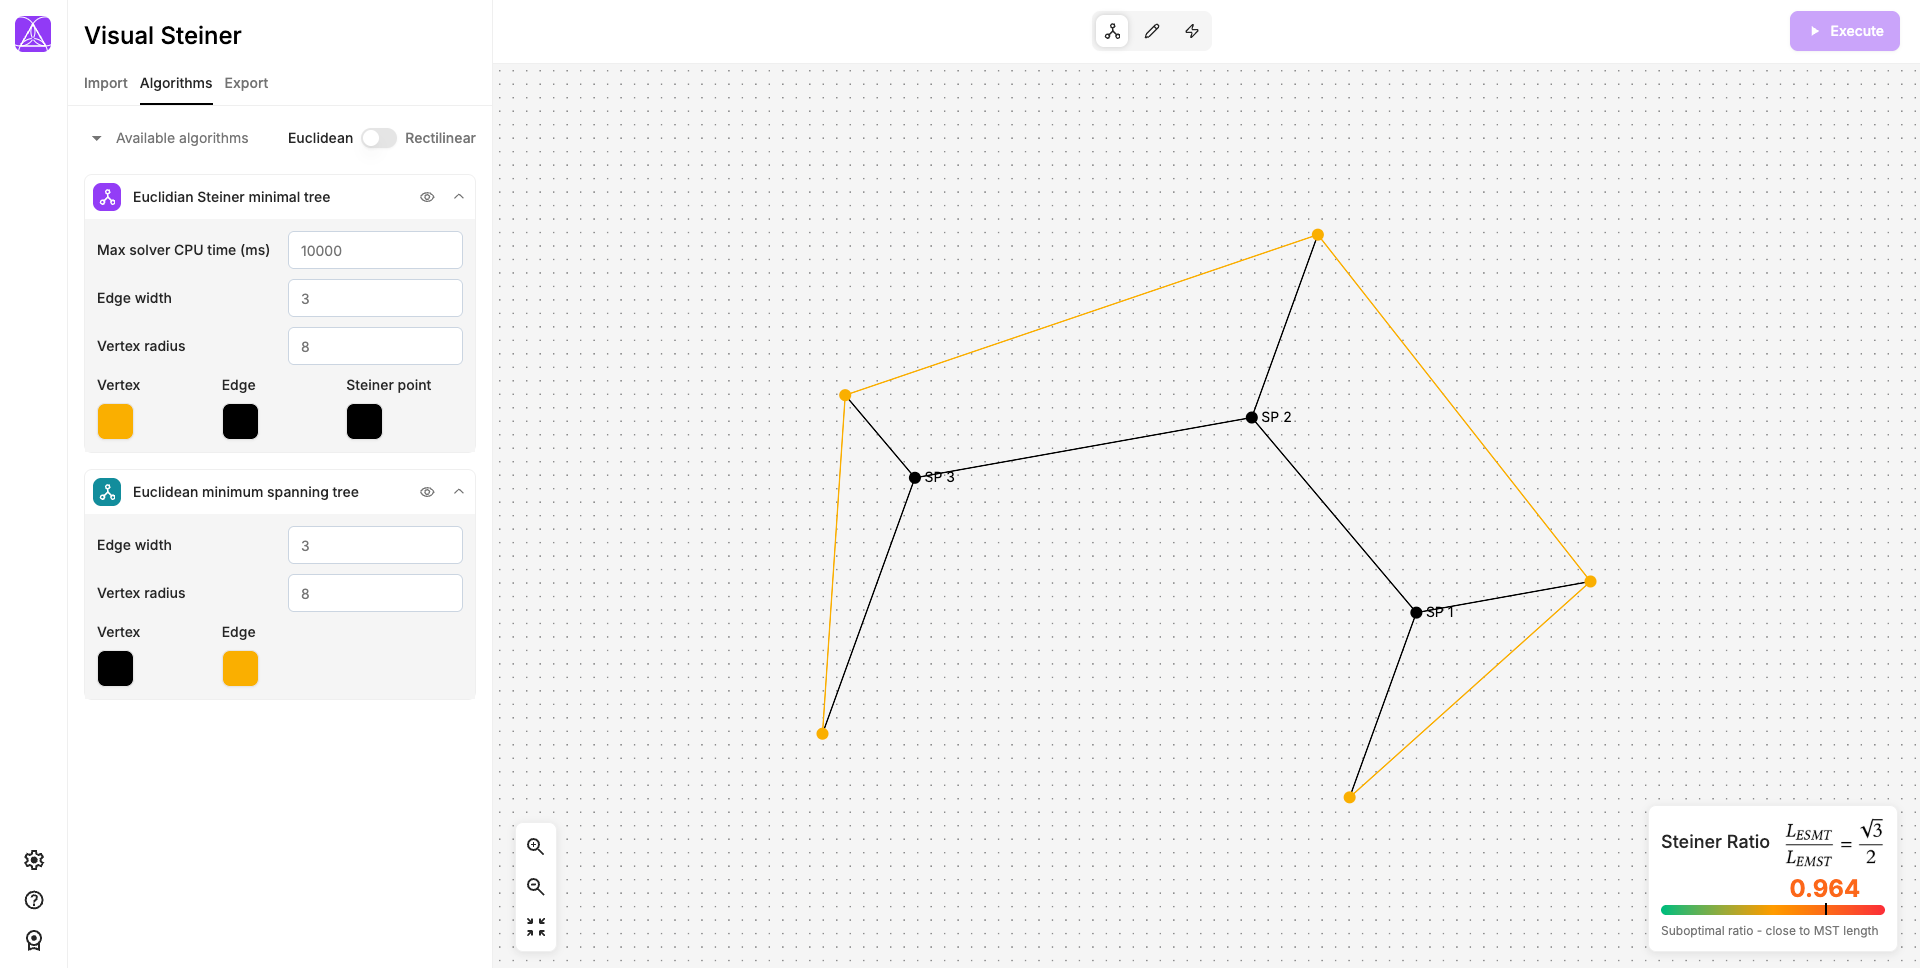
\includegraphics[width=\textwidth]{images/app_overview.png}
    \end{tcolorbox}

    \caption{High-level design of the application.}
    \label{fig:high_level_design}
\end{figure}
Figure \ref{fig:high_level_design} shows the application's design. It features a visual separation between the canvas and the controls (i.e. the sidebar), according to the architecture shown in figure \ref{fig:architecture}.
The canvas takes up most of the screen width since it is expected that most of the user's attention and time will be spent there. The "controls" on the left are partitioned into three sections:
\begin{itemize}
    \item \textbf{Import}: This section displays information about the currently active graph and allows the user to create a new graph, either by importing from a file or by generating a random graph with a specified number of terminals (see section \ref{sec:creating_and_editing_graphs}).
    \item \textbf{Algorithms}: This section contains visualisation customisation options for the output of the algorithms (see section \ref{sec:algorithmic_visualisation}).
    \item \textbf{Export}: This section allows the user to export the currently active graph instance for use in other applications. (see section \ref{sec:exporting_results})
\end{itemize}

As per requirement E1 (see section \ref{sec:requirements}), focus is given to a clean and intuitive design. This is achieved by using a consistent contrastive colour schema, incorporating white space, and using familiar icons to indicate the purpose of the controls.
For example, the two buttons in the centre-top of figure \ref{fig:high_level_design} indicate two "modes" of the canvas. As the right button has a pencil icon, which is commonly used for editing or drawing actions, it is clear that the other button must be for the "non-editing" mode.

Care has also been taken to ensure the primary action is always visible to the user. For instance, the primary action in figure \ref{fig:high_level_design} is the \textit{Execute} button on the top right. Clicking it will recompute the SMT and MST of the currently active graph and display the results on the canvas.
\section{Creating and editing graphs}
\label{sec:creating_and_editing_graphs}

\begin{figure}[hp]
    \centering
    \begin{tcolorbox}[colframe=gray!20, colback=gray!5, boxrule=1pt, arc=0mm, boxsep=0pt, left=0pt, right=0pt, top=0pt, bottom=0pt]
        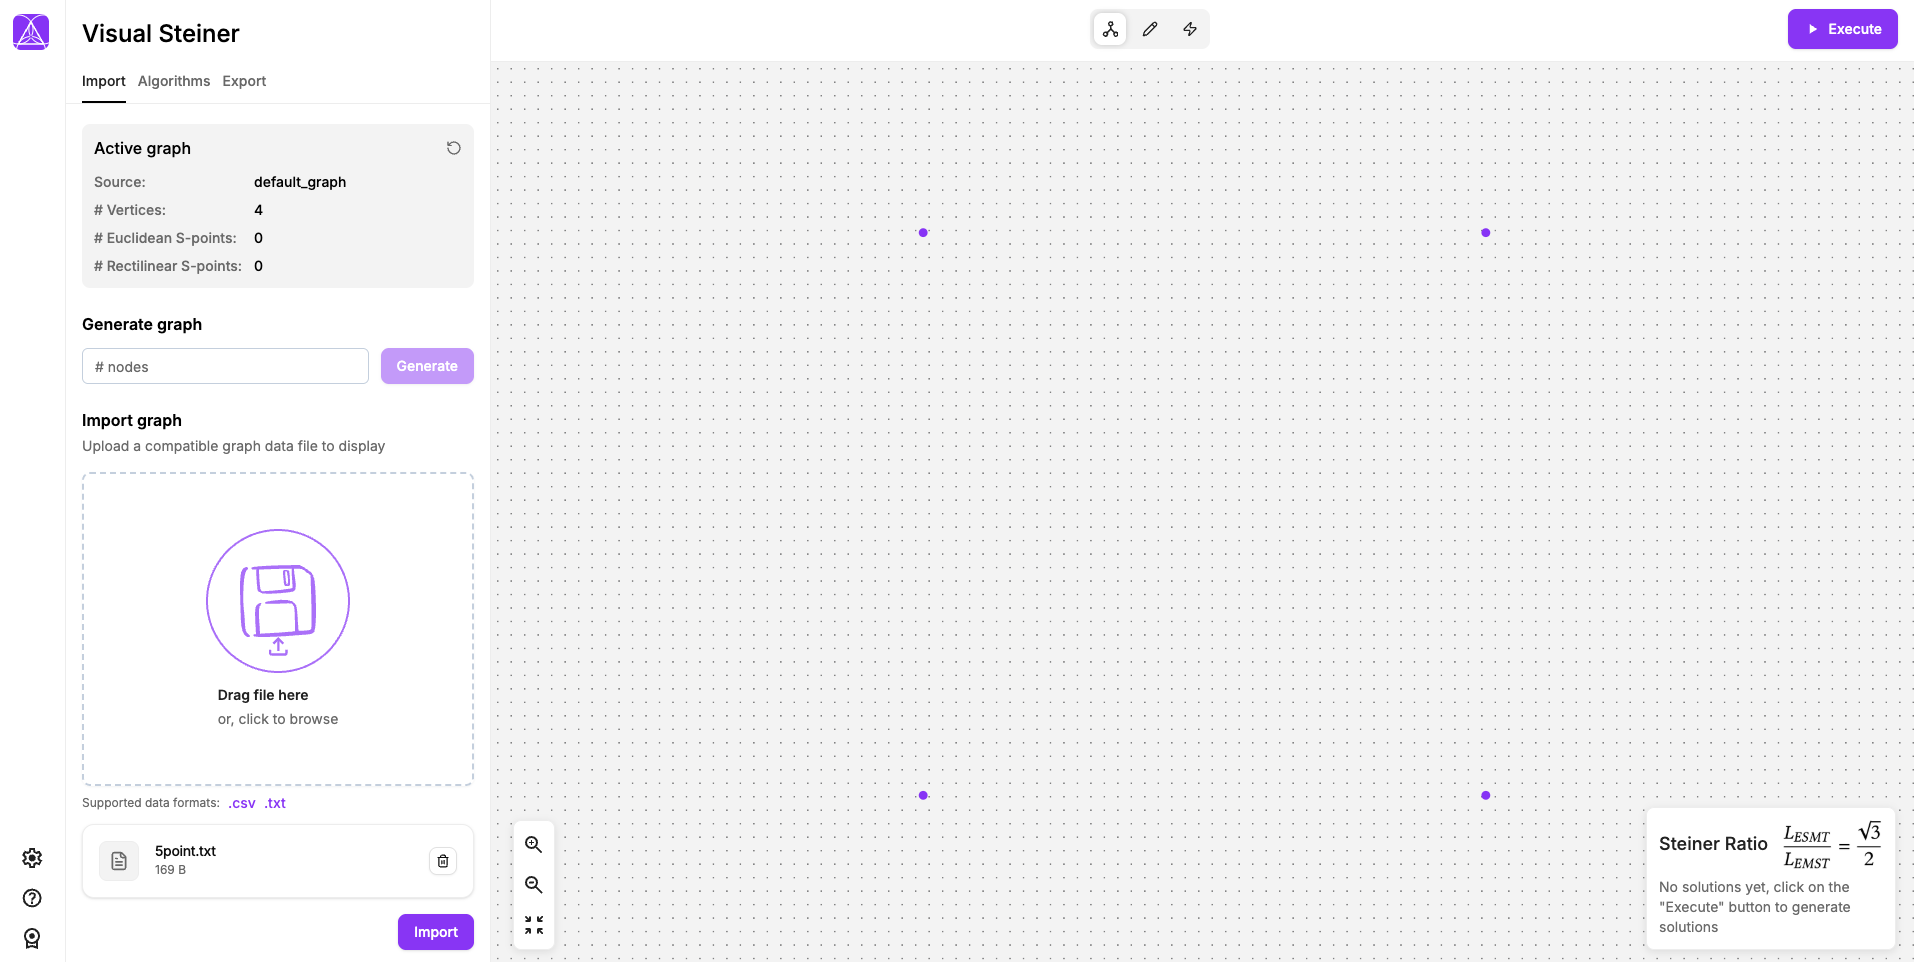
\includegraphics[width=\textwidth]{images/import_view.png}
    \end{tcolorbox}

    \caption{Creating a graph instance by importing from a file or generating a random graph.}
    \label{fig:creating_and_editing_graphs}
\end{figure}
As per requirements E5 and E6 (see section \ref{sec:requirements}), flexibility is given to the user to create or edit graphs at any time in the same view.
The currently active graph instance is displayed at the top of the import tab section in the sidebar (figure \ref{fig:creating_and_editing_graphs}).
The application comes with a default 4-point example graph selected by default.
\subsection{Creating/importing graphs}
Graphs can be created by importing from a file or by generating a random graph with a specified number of terminals.
File formats, such as CSV and TXT, containing a list of 2D coordinates are supported. The user can also download an example file to familiarize themselves with the format.
Again, care has been taken to ensure the primary action is visible. In the example in figure \ref{fig:creating_and_editing_graphs}, the \textit{Import} button is highlighted as a file has been uploaded and is ready to be imported.

\subsection{Editing graphs}
The user can edit the active graph by toggling the \textit{Edit} button in the header above the canvas, which will make the graph in the canvas editable. As all supported algorithms take an undirected, complete graph as input, there was no need for supporting edge drawing. So, the available edit actions have been limited to adding, moving, and removing nodes.

\section{Algorithmic visualisation}
Being able to compare the trees of the MST and SMT algorithms is among the application's main features as per requirement E8 (see section \ref{sec:requirements}). Hence, "layering" was naturally a core design aspect for visualising the algorithmic results. Different layers can be toggled on and off independently, and each layer can be customised with its own set of options (requirements D1 and D3 in \ref{sec:requirements}).
\begin{figure}[hp]
    \centering
    \begin{tcolorbox}[colframe=gray!20, colback=gray!5, boxrule=1pt, arc=0mm, boxsep=0pt, left=0pt, right=0pt, top=0pt, bottom=0pt]
        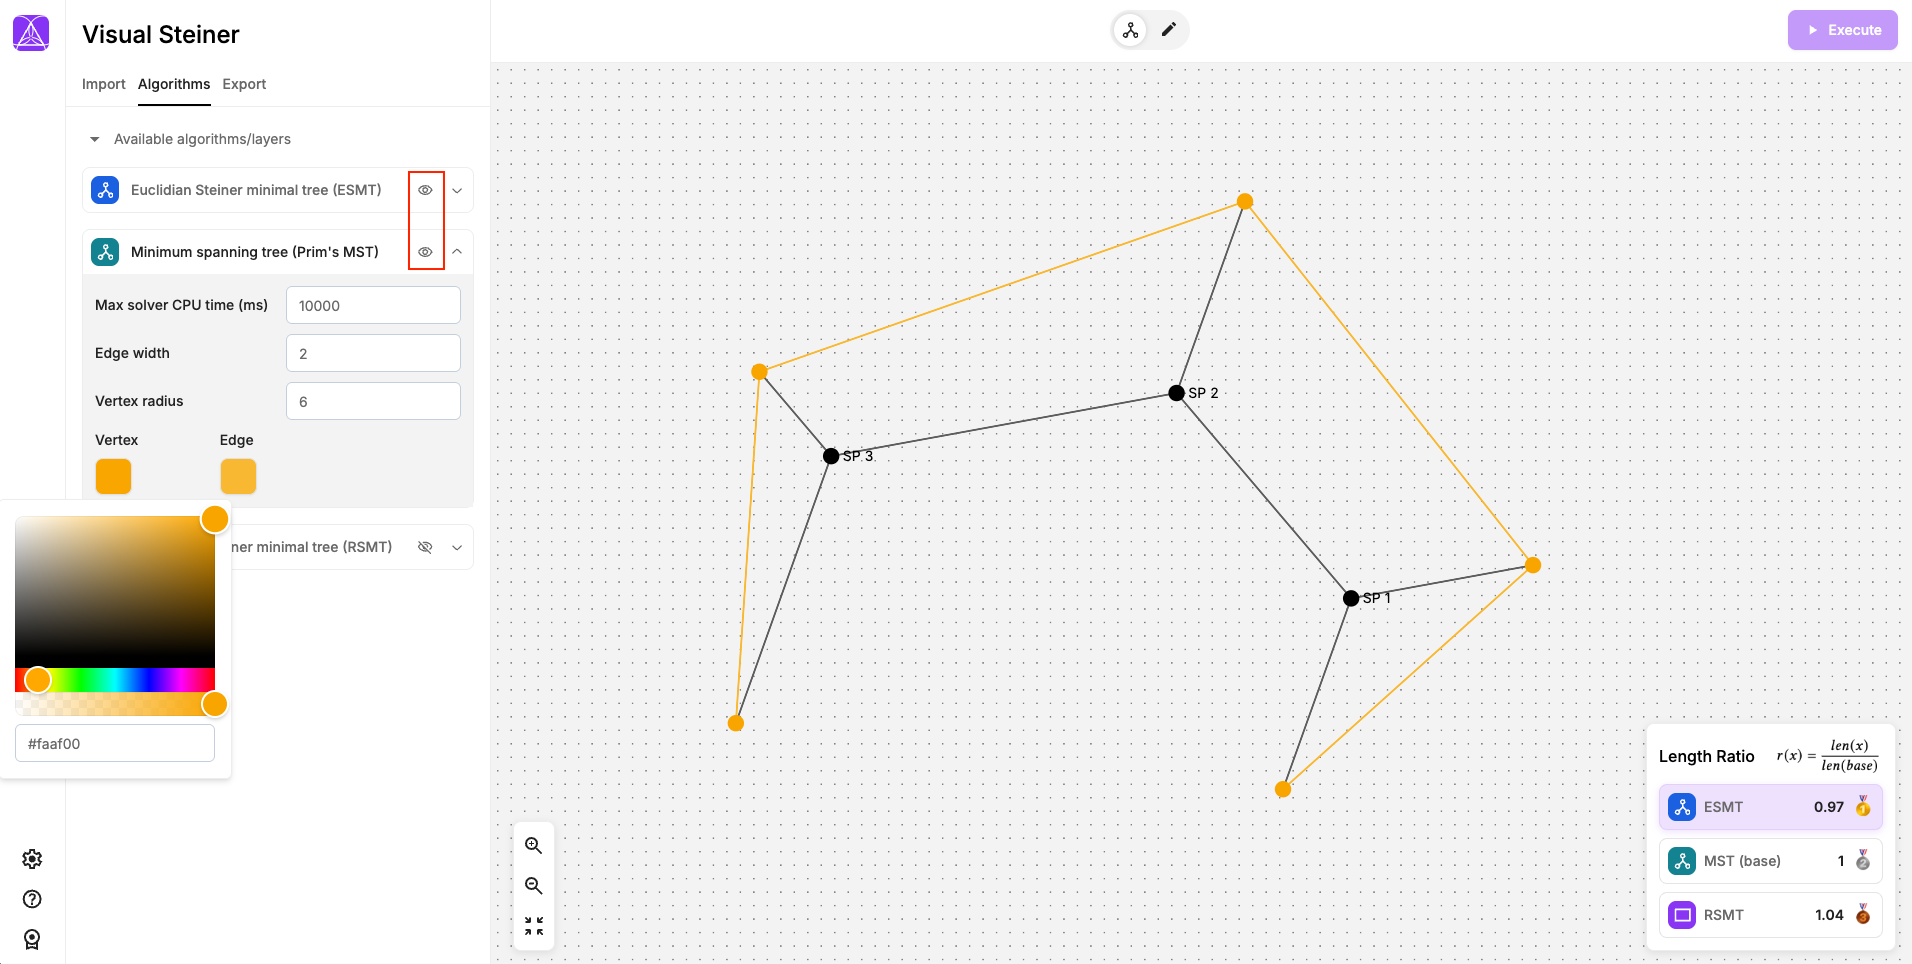
\includegraphics[width=\textwidth]{images/algorithm_visualisation.png}
    \end{tcolorbox}

    \caption{Algorithmic visualisation customisation options showcasing the "layering" approach.}
    \label{fig:algorithm_visualisation}
\end{figure}

\subsection{Layering}
Figure \ref{fig:algorithm_visualisation} shows an example of the algorithmic visualisation customisation options. Both the MST and SMT trees are visible, but their styles can be customised independently. The yellow edges are the MST edges, and the black edges belong to the SMT.

Sometimes, edges or nodes of the two trees overlap. In this case, the hierarchical order of the algorithm layers is used to determine which styles take precedence. In figure \ref{fig:algorithm_visualisation}, the SMT layer is above the MST layer. The terminals are therefore painted with the colour set in the SMT layer (in this case, the colour is the same for both layers).
\subsection{Visualising the Steiner ratio}
As a reminder, the Steiner Ratio is defined as the smallest ratio of the length of the Steiner minimal tree to the length of the minimum spanning tree.
A canvas widget has been added (see bottom left of figure \ref{fig:algorithm_visualisation}) to visualise the Steiner ratio of the currently active graph instance.
This feature is helpful to get an intuition (or potentially find counter-examples) for the Steiner ratio conjecture given by \cite{Gilbert1968SteinerMT}. By dynamically updating the tree and Steiner ratio when the user edits the graph, the user can quickly see how the Steiner ratio changes as the tree changes.

\section{Exporting results}
\label{sec:exporting_results}
The application's usefulness is further enhanced by the ability to export the active graph instance for use in other applications. The export view, shown in figure \ref{fig:exporting_results}, allows the user to export the currently active graph to either an image, like PNG or JPG, or text format, like GEXF\footnote{https://gexf.net/}.
\begin{wrapstuff}[r,width=0.4\textwidth,type=figure]
    \centering
    \begin{tcolorbox}[colframe=gray!20, colback=gray!5, boxrule=1pt, arc=0mm, boxsep=0pt, left=0pt, right=0pt, top=0pt, bottom=0pt]
        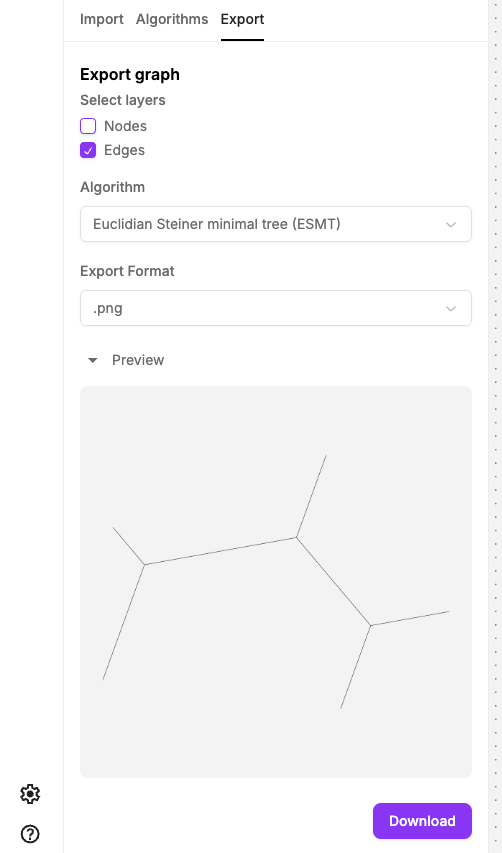
\includegraphics[width=\textwidth]{images/export_view.png}
    \end{tcolorbox}

    \label{fig:exporting_results}
\end{wrapstuff}

Image-based exports are useful for embedding visualisation in other documents, while text-based exports are useful for graphs in other applications. GEXF has been the export format of choice due to its popularity and support for various applications.

When exporting to an image, the user can choose between the customised style set by the user or the default style inspired by how trees are typically visualised in literature. Further, each algorithm's output tree can be exported separately, with the option to render only the edges, nodes, or both.

% The constraining factor for web apps has been the performance of computationally intensive tasks. However, this has been mitigated by the development of WebAssembly (WASM), a technology that allows for near-native performance while still being platform-independent.



\chapter{Analysis of the results}
\label{sec:analysis_results}
As stated in the introduction, the project aimed to develop a fast, accessible, user-friendly interface for visualising Steiner minimal trees and some of their properties.
So far, only the design and implementation of the product have been discussed (see sections \ref{sec:software_design_and_implementation} and \ref{sec:visualisation_and_product_features}), but in this section, the product result is evaluated for its feasibility, how it compares to existing tools, and its potential implications.

\section{Product feasibility}
Requirements E4 and E9 (section \ref{sec:requirements}) stated that product should be deployed as a web application and that it should be able to compute the Steiner minimal tree and Minimum spanning tree of a graph in under 1 second for up to 200 terminals, to be easily accessible and fast. To meet these constraints, instead of building a native app or using the standard client-server architecture, the product was designed as a client-only web application that runs the highly optimised yet computationally expensive GeoSteiner algorithm at near-native speeds directly in the client's browser using WebAssembly.
This section will demonstrate the feasibility of these design choices.

\subsection{Performance}
\label{sec:performance}
By testing the product\footnote{\url{https://steinertree.com}} with multiple random graphs of 200 terminals, it was found that the app was consistently able to compute and render the Steiner minimal tree and Minimum spanning tree of a graph in under a second, meeting the initial design constraints. Naturally, the exact timing will vary depending on the hardware used. Still, the constraint should be interpreted as a rough guideline rather than a strict limit; hence, no quantitative results are included here. Instead, the reader is encouraged to test the product for themselves. Moreover, most use cases are expected to be with graphs much smaller than 200 terminals (see section \ref{sec:implications}). Hence, the product will perform well for most use cases, even on less capable hardware.

The impressively fast performance of the GeoSteiner algorithms has also enabled dynamic tree re-computation when the user edits the graph, meeting requirement E7 (section \ref{sec:requirements}). This feature is only usable and responsive if the computation happens fast enough since long feedback loops will make the UI feel laggy.
\subsection{Ease of access}
As a web application, the product is easily accessible from any device with a modern web browser, and no special tools, installations, or configurations are required. However, the product's UI has not been optimised for mobile screen sizes, as it is expected that most use cases will be on larger screens, such as laptops and desktops.



\section{Comparison with existing tools}
The previous section demonstrated the feasibility of our approach to meeting the performance and accessibility requirements.
This section will discuss how the product compares to existing tools.

Section \ref{sec:existing_tools} listed existing tools and concluded that they lacked a smooth and user-friendly interface, visualisation options, flexible import/export capabilities, and platform independence. A summary of the comparison of features between our product and the existing tools is given in table \ref{tab:tools_comparison}. For a full discussion on the product requirements and features, the reader is referred to sections \ref{sec:requirements} and \ref{sec:visualisation_and_product_features}.

\begin{table}[htbp]
    \centering
    \begin{tabularx}{\textwidth}{l|p{6cm}|p{1.3cm}|p{1.3cm}|p{1.3cm}|p{1.3cm}}
        \textbf{Req.} & \textbf{Feature}                                                                            & STV$^2$            & E3D$^3$   & ST$^4$    & \textbf{Our product} \\
        \midrule
        E1            & Well-designed, clean, and intuitive interface                                               & \ding{55}          & \ding{55} & \ding{51} & \ding{51}            \\
        E2            & Support for the euclidean and rectilinear SMT and MST                                       & \ding{51}          & \ding{55} & \ding{55} & \ding{51}            \\
        E3            & Canvas with large graph, zoom, and pan support                                              & \ding{55}          & \ding{55} & \ding{55} & \ding{51}            \\
        E4            & Computation of 200 nodes < 1 sec                                                            & \ding{55}          & \ding{55} & \ding{55} & \ding{51}            \\
        E5            & Support for flexible graph creation options, including random generation and external files & \ding{55}          & \ding{55} & \ding{55} & \ding{51}            \\
        E6            & Graph can be manipulated on the canvas                                                      & \ding{51}          & \ding{55} & \ding{51} & \ding{51}            \\
        E7            & Dynamic tree updates                                                                        & \ding{51}          & \ding{55} & \ding{51} & \ding{51}            \\
        E8            & Support for comparison of MST/SMT tree structure and length (Steiner Ratio)                 & \ding{51}(partial) & \ding{55} & \ding{55} & \ding{51}            \\
        E9            & Deployed as public web app                                                                  & \ding{55}          & \ding{55} & \ding{55} & \ding{51}            \\
        \midrule
        D1            & Visualisation can be customised                                                             & \ding{55}          & \ding{55} & \ding{55} & \ding{51}            \\
        D2            & Export                                                                                      & \ding{55}          & \ding{55} & \ding{55} & \ding{51}            \\
        D3            & Toggeability of algorithms                                                                  & \ding{51}(partial) & \ding{55} & \ding{55} & \ding{51}            \\
        D4            & Modular and extensible software architecture                                                & \ding{55}          & -         & \ding{55} & \ding{51}            \\
    \end{tabularx}
    \caption{Feature comparison between the existing tools and the end product. See the requirements section \ref{sec:requirements} for more details.}
    \label{tab:tools_comparison}
\end{table}
\footnotetext[2]{\url{https://github.com/Keydrain/Steiner-Tree-Visualisation}}
\footnotetext[3]{\url{https://github.com/Kallel-Abd/ESteiner-3D}}
\footnotetext[4]{\url{https://github.com/Dawkey/Steiner-Tree}}


\section{Implications}
\label{sec:implications}
In this section, the implications of the result will be discussed. As shown in figure \ref{fig:architecture}, the application is split into two main components, the GeoSteiner WASM module and the UI. Each component has its own set of implications, which will be discussed in the following sections.
\subsection{Wider use of the GeoSteiner WASM module}

As mentioned in section \ref{sec:geosteiner_integration}, the GeoSteiner WASM module is a portable byte code representation of the GeoSteiner algorithms library implemented in C. Due to WASM's portability and highly efficient byte code organisation, it is now feasible to use the GeoSteiner algorithm in any language that supports WASM. In other words, integrating with the GeoSteiner algorithms became much easier. This opens the door for usage of the GeoSteiner algorithms in other applications, such as network analysis libraries\footnote[5]{\url{https://networkx.org}}. These libraries often rely on approximate algorithms as it is hard to implement an efficient version of an exact Steiner tree algorithm.

Moreover, as the GeoSteiner WASM module is entirely independent of the UI, it could be used in other (open source) graph visualisation tools, such as GeoGebra \footnote[6]{\url{https://www.geogebra.org/geometry}}.
\subsection{Using the visualisation tool in research}
The visualisation tool may also have several uses in research. First, its features will be useful for gaining a better intuition for the Steiner tree and its properties. For instance, our implementation can smoothly recompute the Steiner minimal tree in response to user input, such as adding, moving, or removing points. This enables the user to observe how the Steiner ratio changes as a function of the configuration of the terminals. It also allows verifying potential counter-examples to the (Euclidean) Steiner ratio conjecture in real time.

%==================================================================================================================================
\chapter{Conclusion}
\label{sec:conclusion}
\section{Summary of the problem}
The Steiner minimal tree (SMT) problem and the minimum spanning tree (MST) problem belong to the class of network optimisation problems. The SMT problem is similar to the MST problem but allows for the addition of Steiner points to further reduce the tree length.
Despite being simple to state, the SMT problem is NP-hard. Consequently, its associated exponential complexity has limited the feasibility and practicality of visualisation tools, in contrast to the MST problem, which has efficient algorithms and plenty of visualisation options. This lack has also limited the ability of researchers and students to build an intuition for the problem, particularly in investigating the Steiner ratio (still an open problem in the Euclidean but not in the rectilinear case), which is the smallest ratio of the length of the Steiner minimal tree to the length of the Minimum spanning tree.

\section{Summary of contributions}
This dissertation presented the development of a web-based visualisation tool for the Euclidean and rectilinear variants of the Steiner minimal tree and Minimum spanning tree. The tool leverages GeoSteiner, the fastest known algorithm for the SMT problem, and exploits state-of-the-art techniques for optimal performance.
The result is a publicly available client-only web app\footnote{\url{https://steinertree.com}} that can be run on any device with a modern web browser.

The \textbf{key contributions} of this work include:
\begin{itemize}
    \item The first successful (open source) compilation of the GeoSteiner implementation to WebAssembly. With this, the GeoSteiner algorithm is now easily accessible to any programming language that supports WASM.
    \item The first publicly available online visualisation tool for the Steiner minimal and minimum spanning trees.
    \item A fast and interactive interface allows the user to compute and visualise the Steiner minimal tree and Minimum spanning tree of any graph instance and compare them in structure and length. Despite the theoretical exponential complexity of the SMT problem, the tool can compute and display the results for graphs with up to 200 terminals in sub-second times.
    \item A dynamic tree-updating feature enables the user to observe how the Steiner ratio changes in real time as the graph is edited.
\end{itemize}

The abstraction of the GeoSteiner implementation to a WebAssembly module makes integration into new programming languages and applications straightforward. This opens new possibilities and could lead to the broader adoption of exact algorithms instead of approximations in open source network analysis libraries and other geometric computing or visualisation tools.
Moreover, researchers could use the visualisation tool to explore the Steiner tree and its properties in a new and interactive way. In particular, the dynamic tree-updating feature has dramatically reduced the feedback loop for investigating potential counter-examples to the Steiner ratio conjecture.

\section{Future work}
This section discusses potential future work for the GeoSteiner WASM module and the visualisation tool.

\subsection{GeoSteiner WASM module}
The GeoSteiner WASM module could be extracted into a separate package and distributed as a stand-alone library in the JavaScript ecosystem through NPM. This would make it easier to integrate it into other web-based applications, such as GeoGebra. Different language bindings could also be created for the GeoSteiner WASM module and distributed as separate packages in the package manager of choice for each programming language.

\subsection{Visualisation tool}
The visualisation tool has the potential to be extended with new graph algorithms and could serve as a general-purpose tool for visualising and analysing graphs.
In addition, several optimisations could be applied to improve the tool's performance even further. For example, the algorithms' computation could be moved to another Web-worker thread to avoid blocking the browser's main thread.
The UI itself could also benefit from improvements, such as adding a responsive design for mobile devices and canvas support for bent edges, which is especially relevant for visualising the rectilinear Steiner minimal tree.

\begin{appendices}

    \chapter{Melzak algorithm complexity derivation}
    \label{app:melzak_complexity}

    \todo{State where we got this from, why we included the derivation and what are our contributions}
    The formula derivation for the number of full topologies $F^*(n)$ based on Property 7 in \cite{Gilbert1968SteinerMT} is given below.

    Let $f(s)$ be the number of full topologies for the case of $s$ Steiner points.
    Let $F(n, s)$ be the number of (non-full) topologies for the case of $n$ terminals and $s$ Steiner points. $F(n, s)$ can be written in terms of $f(s)$ as follows.

    If we assume that Steiner points are unlabeled, there are $\binom{n}{s+2}$ ways to choose the terminals from which the full topology will be constructed. Each chosen set of terminals has $f(s)$ possible full topologies. Hence, there are a total of $\binom {n}{s+2}f(s)$ possible full topologies.

    There are still $n - (s + 2)$ points left, which can be added to the currently full topology to make it non-full. A tree has $n - 1$ edges, hence the current full topology has $((s + 2) + s) - 1 = 2s + 1$ edges. The leftover points can be added by splitting existing edges into two, resulting in the net addition of 1 edge.

    For the first leftover point, we have $2s + 1$ possible edges to split, for the second $2s + 2$, and so on. This is repeated until the last leftover point is added; at this point, our topology has $n + s - 1$ edges. This can be written as
    \begin{equation*}
        \begin{aligned}
            F(n, s) & = \binom{n}{s+2}f(s)(2s + 1)(2s + 2)\cdots(n + s - 2) \\
                    & = \binom{n}{s+2}f(s)\frac{(n + s - 2)!}{(2s)!}
        \end{aligned}
    \end{equation*}

    The formula for $f(s)$ can be defined recursively as follows:
    \begin{equation*}
        \begin{aligned}
            f(0)   & = 1            \\
            f(s+1) & = (2s + 1)f(s)
        \end{aligned}
    \end{equation*}
    In other words, when all $f(s)$ full topologies are found, adding one more Steiner point by the same edge-splitting technique to each of the $f(s)$ topologies results in $(2s + 1)f(s)$ new topologies.
    This recurrence relation can be solved by using the double-factorial form for an odd integer $n = 2k - 1$, with $k \ge 0$ \citep{Double_factorial}.
    $$
        (2k - 1)!! = \frac{(2k)!}{2^k k!}
    $$
    Rewriting $f(s)$ in terms of the double-factorial, we get
    $$
        f(s) = \frac{(2s)!}{2^{s}(s)!}
    $$

    Finally,
    \begin{equation*}
        \begin{aligned}
            F(n, s) & = \binom{n}{s+2}\frac{\cancel{(2s)!}}{2^s(s)!}\frac{(n + s - 2)!}{\cancel{(2s)!}} \\
                    & = \binom{n}{s+2}\frac{(n + s - 2)!}{2^s(s)!}
        \end{aligned}
    \end{equation*}

    In the case of the Melzak algorithm, only full topologies are considered. We therefore let $n = k$ and $s = k - 2$, and rewrite $F(n, s)$ to $F(n)$.
    \begin{equation*}
        \begin{aligned}
            F(n) = \binom{n}{k}\frac{(2k - 4)!}{2^{k-2}(k-2)!}
        \end{aligned}
    \end{equation*}

    Since the full topologies are considered for all subsets of $n$ terminals, starting from 2 terminals as the Minimum, we arrive at the original expression.
    \begin{equation*}
        \begin{aligned}
            F^*(n) = \sum_{k=2}^{n} \binom{n}{k}\frac{(2k - 4)!}{2^{k-2}(k-2)!}
        \end{aligned}
    \end{equation*}

    \chapter{Codebase structure}
    \label{app:repository_structure}
    \begin{table}[h]
    \centering

    % Make colors lighter (20% opacity)
    \definecolor{reactLight}{RGB}{207, 241, 253}     % React light blue at 20%
    \definecolor{typescriptLight}{RGB}{194, 213, 236}  % TypeScript blue at 20%
    \definecolor{cLight}{RGB}{207, 225, 243}         % C blue at 20%
    \definecolor{wasmLight}{RGB}{211, 194, 222}      % WASM purple at 20%
    \definecolor{testLight}{RGB}{247, 204, 211}      % Test red at 20%
    \definecolor{staticLight}{RGB}{211, 225, 206}    % Static assets green at 20%

    \begin{tabular}{|p{5cm}|p{1.5cm}|p{6cm}|p{1cm}|}
        \hline
        \rowcolor{white} % Make sure header row is white
        \textbf{Asset}                        & \textbf{Type} & \textbf{Description}                                                                                                                                               & \textbf{LOC} \\
        \hline
        \rowcolor{reactLight}
        src/components/*                      & React         & Collection of reusable React components based on Shadcn/UI.                                                                                                        & 1030         \\
        \hline
        \rowcolor{reactLight}
        src/features/*                        & React         & Features are independent modules that have a specific scope and their own set of components, hooks, types, and tests. Features include the canvas and the sidebar. & 2210         \\
        \hline
        \rowcolor{reactLight}
        src/hooks/*                           & React         & Collection of global custom function hooks for functionality such as pub-sub, debouncing, sorted lists, etc.                                                       & 68           \\
        \hline
        \rowcolor{reactLight}
        src/providers/*                       & React         & Collection of scoped state management providers                                                                                                                    & 231          \\
        \hline
        \rowcolor{reactLight}
        index.html, src/main.tsx, src/App.tsx & React         & Entry point for the web application.                                                                                                                               & 53           \\

        \hline
        \rowcolor{typescriptLight}
        src/lib/*                             & Typescript    & Contains all business logic for the application, such as algorithms, data structures, utilities, input parsers, etc.                                               & 585          \\
        \hline
        \rowcolor{cLight}
        geosteiner/*                          & C             & Contains a copy of the open source GeoSteiner library with some modifications for compatibility with WASM.                                                         & n/a          \\
        \hline
        \rowcolor{wasmLight}
        wasm/*                                & WASM          & Contains the setup for compiling the GeoSteiner library into a WASM module and the simplified GeoSteiner API for the calling code.                                 & 79           \\
        \hline
        \rowcolor{testLight}
        **/tests/*                            & Typescript    & Integration/unit tests across the codebase.                                                                                                                        & 301          \\
        \hline
        \rowcolor{staticLight}
        public/*                              & Static assets & Static assets such as images, icons, examples, and the WASM module.                                                                                                & N/A          \\
        \hline
    \end{tabular}
    \caption{Repository structure and distribution of code. Only the important folders are listed. The LOC values are accurate as of 28/03/2025.}
    \label{tab:project_structure}
\end{table}



\end{appendices}

% The bibliography style is agsm (Harvard)
% The bibliography always appears last, after the appendices.

\bibliographystyle{agsm}

% Force the bibliography not to be numbered
\renewcommand{\thechapter}{0}
\bibliography{l4proj}

\end{document}